%==============================================================================
% Education and Employment Exits During COVID-19: Evidence from Brazil
% Cavalcanti, Didier and Gonzaga
%
% Prepared for Labour Economics (Elsevier), elsarticle class.
% Compile with:  latexmk -pdf paper.tex   (run from the latex/ directory)
%
% Tables, figures and every number quoted in the text are produced by the R
% pipeline in analysis/code and are read from ../analysis/output. Nothing
% numeric is hard-coded here; see README.md.
%==============================================================================

\documentclass[review,3p,authoryear]{elsarticle}

\usepackage[T1]{fontenc}
\usepackage[utf8]{inputenc}
\usepackage{lmodern}
\usepackage{microtype}
\usepackage{amsmath, amssymb}
\usepackage{booktabs}
\usepackage{graphicx}
\usepackage{threeparttable}
\usepackage{float}
\usepackage{xcolor}
\usepackage[colorlinks=true]{hyperref}
% House colour for citations and links, as in the HomeOfficePNAD and HealthEcon
% projects.
\definecolor{citegreen}{RGB}{0,120,60}
% elsarticle.cls forces \@linkcolor/\@citecolor/\@urlcolor to blue inside its
% own \AtBeginDocument hook, so preamble options are overwritten. It sets those
% internals with \def rather than \hypersetup, and a late \hypersetup cannot
% re-enable colouring once the class has run, so we override the same internals
% in a hook registered after the class's.
\makeatletter
\AtBeginDocument{%
  \def\@linkcolor{citegreen}%
  \def\@citecolor{citegreen}%
  \def\@urlcolor{citegreen}%
  \def\@filecolor{citegreen}%
}
\makeatother

\graphicspath{{../analysis/output/figures/}}

\journal{Labour Economics}

% Estimates and sample counts quoted in the text (auto-generated).
% Auto-generated by analysis/code/09_paper_numbers.R. Do not edit by hand.
\newcommand{\Nobs}{7,764,610}
\newcommand{\Nind}{2,922,141}
\newcommand{\Npsu}{39,251}
\newcommand{\Nhh}{1,620,032}
\newcommand{\Nquarters}{52}
\newcommand{\QfirstLab}{2012Q1}
\newcommand{\QlastLab}{2024Q4}
\newcommand{\RawExit}{9.4}
\newcommand{\RawExitNoCol}{10.7}
\newcommand{\RawExitCol}{4.0}
\newcommand{\ShareCollege}{20}
\newcommand{\ShareInformal}{40}
\newcommand{\RawExitFormal}{4.9}
\newcommand{\RawExitInformal}{16.1}
\newcommand{\RawExitEU}{2.9}
\newcommand{\RawExitEN}{6.5}
\newcommand{\NoriginsAll}{11,491,554}
\newcommand{\MatchRateAll}{84.2}
\newcommand{\PreGap}{-0.008}
\newcommand{\PreGapSE}{0.001}
\newcommand{\PreGapPP}{-0.8}
\newcommand{\PreGapLo}{-0.010}
\newcommand{\PreGapHi}{-0.005}
\newcommand{\PreLevNoCol}{0.099}
\newcommand{\PreLevCol}{0.092}
\newcommand{\OnsetGap}{-0.035}
\newcommand{\OnsetGapSE}{0.001}
\newcommand{\OnsetGapPP}{-3.5}
\newcommand{\OnsetGapLo}{-0.037}
\newcommand{\OnsetGapHi}{-0.032}
\newcommand{\OnsetLevNoCol}{0.136}
\newcommand{\OnsetLevCol}{0.101}
\newcommand{\MidGap}{0.018}
\newcommand{\MidGapSE}{0.001}
\newcommand{\MidGapPP}{1.8}
\newcommand{\MidGapLo}{0.016}
\newcommand{\MidGapHi}{0.021}
\newcommand{\MidLevNoCol}{0.056}
\newcommand{\MidLevCol}{0.075}
\newcommand{\PostGap}{-0.009}
\newcommand{\PostGapSE}{0.001}
\newcommand{\PostGapPP}{-0.9}
\newcommand{\PostGapLo}{-0.011}
\newcommand{\PostGapHi}{-0.006}
\newcommand{\PostLevNoCol}{0.096}
\newcommand{\PostLevCol}{0.087}
\newcommand{\PreGapAbsPP}{0.8}
\newcommand{\MidGapAbsPP}{1.8}
\newcommand{\OnsetRelNoCol}{37}
\newcommand{\OnsetRelCol}{10}
\newcommand{\MidRelNoCol}{-43}
\newcommand{\MidRelCol}{-18}
\newcommand{\MidRelNoColAbs}{43}
\newcommand{\MidRelColAbs}{18}
\newcommand{\SuptCrit}{2.73}
\newcommand{\NRevQuarters}{7}
\newcommand{\RevFirst}{2013Q3}
\newcommand{\RevLast}{2021Q3}
\newcommand{\NRevSimQuarters}{6}
\newcommand{\GapOnsetQ}{-0.035}
\newcommand{\GapMaxRev}{0.024}
\newcommand{\GapMaxRevQ}{2021Q2}
\newcommand{\FormalMidGap}{0.002}
\newcommand{\FormalPreGap}{-0.009}
\newcommand{\FormalMidGapSE}{0.001}
\newcommand{\InformalMidGap}{0.020}
\newcommand{\InformalPreGap}{-0.012}
\newcommand{\InformalMidGapSE}{0.002}
\newcommand{\MenMidGap}{0.016}
\newcommand{\MenPreGap}{-0.003}
\newcommand{\WomenMidGap}{0.028}
\newcommand{\WomenPreGap}{-0.009}
\newcommand{\WhiteMidGap}{0.011}
\newcommand{\WhitePreGap}{-0.008}
\newcommand{\NonWhiteMidGap}{0.022}
\newcommand{\NonWhitePreGap}{-0.012}
\newcommand{\InfSelfMidGap}{0.000}
\newcommand{\InfPrivMidGap}{0.029}
\newcommand{\InfPrivPreGap}{-0.012}
\newcommand{\FormPrivMidGap}{0.001}
\newcommand{\FormSelfMidGap}{0.007}
\newcommand{\FormPubMidGap}{-0.003}
\newcommand{\DecPreTotal}{-0.069}
\newcommand{\DecPreComp}{-0.038}
\newcommand{\DecPreWithin}{-0.031}
\newcommand{\DecPreCompShare}{55}
\newcommand{\DecPreWithinShare}{45}
\newcommand{\DecOnsetTotal}{-0.090}
\newcommand{\DecOnsetComp}{-0.045}
\newcommand{\DecOnsetWithin}{-0.046}
\newcommand{\DecOnsetCompShare}{49}
\newcommand{\DecOnsetWithinShare}{51}
\newcommand{\DecMidTotal}{-0.040}
\newcommand{\DecMidComp}{-0.021}
\newcommand{\DecMidWithin}{-0.019}
\newcommand{\DecMidCompShare}{53}
\newcommand{\DecMidWithinShare}{47}
\newcommand{\DecPostTotal}{-0.068}
\newcommand{\DecPostComp}{-0.035}
\newcommand{\DecPostWithin}{-0.034}
\newcommand{\DecPostCompShare}{51}
\newcommand{\DecPostWithinShare}{49}
\newcommand{\DecWithinShrink}{39}
\newcommand{\DecCompShrink}{44}
\newcommand{\DecRawShrink}{42}
\newcommand{\RetOverall}{0.851}
\newcommand{\RetDiffPre}{0.021}
\newcommand{\RetDiffMid}{0.048}
\newcommand{\RetDiffOnset}{0.077}
\newcommand{\RetColMid}{0.855}
\newcommand{\RetNoColMid}{0.807}
\newcommand{\IpwMidGap}{0.019}
\newcommand{\IpwMidGapSE}{0.001}
\newcommand{\BaseMidGap}{0.018}
\newcommand{\IpwMidGapFour}{0.0188}
\newcommand{\BaseMidGapFour}{0.0184}
\newcommand{\PlaceboTau}{0.0271}
\newcommand{\PlaceboSE}{0.0018}
\newcommand{\PlaceboP}{0.000}
\newcommand{\PlaceboNPre}{27}
\newcommand{\PlaceboNGE}{0}
\newcommand{\PlaceboPPlacebo}{0.036}
\newcommand{\OverlapMidGap}{-0.005}
\newcommand{\BaseOverlapMidGap}{0.018}
\newcommand{\OverlapInfMidGap}{-0.007}
\newcommand{\BaseOverlapInfMidGap}{0.020}
\newcommand{\OverlapOffSupport}{17.0}
\newcommand{\OverlapMidGapOff}{17}
\newcommand{\OverlapInfOffSupport}{31.6}
\newcommand{\OverlapEssRatio}{32}
\newcommand{\TrimPreGap}{-0.008}
\newcommand{\TrimMidGap}{-0.003}
\newcommand{\TrimMidSE}{0.001}
\newcommand{\TrimInfPreGap}{-0.016}
\newcommand{\TrimInfMidGap}{0.001}
\newcommand{\TrimInfMidSE}{0.004}
\newcommand{\TrimShare}{28}
\newcommand{\TrimInfShare}{14}
\newcommand{\TippingDelta}{none}
\newcommand{\TippingRateMAR}{0.040}
\newcommand{\TippingRateAt}{--}
\newcommand{\TippingFloor}{0.013}
\newcommand{\TippingDeltaMin}{-8}
\newcommand{\RealocCollege}{0.0035}
\newcommand{\RealocNonCollege}{0.0004}
\newcommand{\RealocShare}{20}
\newcommand{\DecVarCompLo}{-0.021}
\newcommand{\DecVarCompHi}{-0.020}
\newcommand{\PreGapInf}{-0.027}
\newcommand{\MidGapInf}{-0.045}
\newcommand{\MidGapEU}{0.001}
\newcommand{\MidGapEUSE}{0.001}
\newcommand{\PreGapEU}{-0.002}
\newcommand{\MidGapEN}{0.017}
\newcommand{\MidGapENSE}{0.001}
\newcommand{\PreGapEN}{-0.006}
\newcommand{\WcbOnset}{0.149}
\newcommand{\WcbMid}{$<$0.0001}
\newcommand{\BWild}{9,999}
\newcommand{\BSupt}{10,000}
\newcommand{\BDecomp}{2,000}
\newcommand{\Seed}{20260615}


\newcommand{\jelcodes}[1]{\textit{JEL classification:} #1}

% elsarticle defines \appendixname as "Appendix " with a trailing space and then
% builds \thesection as "\appendixname~\Alph{section}", so both the appendix
% headings and every \ref to one come out with two spaces: "Appendix  A".
% Dropping the trailing space leaves the tie as the single separator.
\renewcommand{\appendixname}{Appendix}
% The tie is still ordinary interword glue, which justification can stretch.
% \mbox freezes it at its natural width and keeps the two halves on one line.
\newcommand{\appref}[1]{\mbox{\ref{#1}}}

\begin{document}

\begin{frontmatter}

\title{Education and Employment Exits During COVID-19:\\ Evidence from Brazil}

\author[ufpe]{Francisco Cavalcanti}
\ead{francisco.dlcavalcanti@ufpe.br}
\affiliation[ufpe]{organization={PIMES, Federal University of Pernambuco (UFPE)},
  city={Recife}, state={PE}, country={Brazil}}

\author[idp]{Fredie Didier\corref{cor}}
\ead{fdidier@terra.com.br}
\cortext[cor]{Corresponding author.}
\affiliation[idp]{organization={Instituto Brasileiro de Ensino, Desenvolvimento e Pesquisa (IDP)},
  city={Bras\'ilia}, state={DF}, country={Brazil}}

\author[puc]{Gustavo Gonzaga}
\ead{gonzaga@econ.puc-rio.br}
\affiliation[puc]{organization={Department of Economics, PUC-Rio},
  city={Rio de Janeiro}, state={RJ}, country={Brazil}}

\begin{abstract}
We use the rotating panel of Brazil's \textit{PNAD Cont\'inua} to ask how the
education gradient in the risk of leaving employment moved through the COVID-19
pandemic. Linking \Nind{} workers across \Nquarters{} quarters
(\QfirstLab--\QlastLab, \Nobs{} person-quarters), we estimate survey-weighted
average predictive margins for workers with and without a college degree,
quarter by quarter. Unconditionally the gradient is large and never reverses:
graduates leave employment at \RawExitCol\% per quarter against
\RawExitNoCol\%. Once we hold constant where people work, it does. Over six
consecutive quarters, from 2020Q2 to 2021Q3, college graduates were
\MidGapAbsPP{} percentage points more likely to leave employment than
otherwise comparable non-graduates, before the pre-pandemic gradient returned.
A decomposition locates the result. Composition, meaning that graduates hold
different jobs, and within-cell risk contribute about equally in every period,
and during
the window both compress by roughly \DecWithinShrink\%, so the raw gap halves
without changing sign. The reversal appears only once workers are matched on pay,
hours, tenure and contract type as well, and it is concentrated among informal
private employees. Splitting the outcome by destination places it entirely on
one margin: the reversal is a movement out of the labour force, not into
measured unemployment. Retention in the panel is
stable across education groups, and weighting by the inverse probability of
being re-interviewed leaves the result unchanged. The episode shows how
emergency support segmented along the formal--informal margin can temporarily
detach job security from schooling.
\end{abstract}

\begin{keyword}
Employment exits \sep Education \sep Informality \sep COVID-19 \sep Brazil
\sep Rotating panel
\end{keyword}

\end{frontmatter}

\noindent\jelcodes{J63, J24, J46, I38, O17}

%==============================================================================
\section{Introduction}
%==============================================================================

Job security rises with schooling. Across the OECD, unemployment among workers
with tertiary education averages 4--5\%, against 12.8\% for those without upper
secondary education.\footnote{OECD (2023), \textit{Education at a Glance 2023}.}
The COVID-19 recession initially widened that gradient almost everywhere: in the
United States, unemployment among workers with at most a high school diploma
rose by 11 percentage points between February and May 2020, three times the
increase recorded for college graduates \citep{Pew2020, Montenovo2022,
Cajner2020}, and the incidence of the shock was sharply unequal along skill
lines more generally \citep{Prassl2020, Albanesi2021, Aum2021}.

The mechanisms are familiar. Human capital raises productivity and lowers
displacement risk \citep{BenPorath1967, Mincer1974, Lise2020}; education sorts
workers into more stable jobs and cushions them against cyclical downturns
\citep{Farber2005, Hoynes2012}, into activities less exposed to reallocation
shocks \citep{Davis1987, Brainard1993}, and into tasks more amenable to remote
work \citep{Autor2003, Dingel2020, Barrero2023}. Causal evidence is scarcer, but
\citet{Beuermann2024} exploit school-assignment discontinuities in Barbados and
find that additional schooling did reduce the probability of losing a job after
the COVID-19 onset, in a way their evidence attributes to skill rather than to
signalling or to sectoral sorting.

This paper asks whether that gradient held in a labour market where two in five
workers are informal and where the emergency policy response was explicitly
segmented along the formal--informal margin. Brazil is an informative case
precisely because its two main interventions worked through different parts of
the labour market. \textit{Aux\'ilio Emergencial}, a large cash transfer, paid
monthly benefits from April 2020 through October 2021 and reached informal and
low-income workers \citep{Arruda2022, Neri2020, Lopez2023}. In parallel, the
\textit{Programa Emergencial de Manuten\c{c}\~ao do Emprego e da Renda} let
formal employers cut hours and wages or suspend contracts with partial income
replacement \citep{MTE2020}. Because schooling and formality are strongly
correlated \citep{Ulyssea2020, Parente2024}, the two programmes did not simply
differ in generosity: they reached different education groups.

A substantial literature already documents the aggregate contraction of
Brazilian and Latin American employment during COVID-19 and the disproportionate
exposure of informal workers. \citet{Maurizio2023} show, for six Latin American
countries including Brazil, that the fall in informal employment drove the
overall contraction, that it operated mainly through higher exit rates rather
than lower entry, and that most informal workers who lost their jobs left the
labour force altogether. \citet{Bottan2020} document unequal exposure across
seventeen developing countries, and work on \textit{Aux\'ilio Emergencial}
establishes both its coverage and its behavioural effects \citep{Arruda2022,
Lopez2023, Andrade2021}. What this literature has not established is whether
schooling itself continued to protect workers once the composition of jobs is
held fixed. Nor, if it did not, whether that reflects a change in where graduates
and non-graduates work or a change in the risk they face inside the same kind of
job.

That is our contribution. We provide longitudinal evidence on quarterly
employment exits by education over \QfirstLab--\QlastLab, and we show whether
the temporary reversal of the education gradient reflects changes in workforce
composition or changes in within-cell transition risks, particularly within
informal employment. Three features of the exercise matter. First, we report
survey-weighted average predictive margins for each education-by-quarter cell
and the corresponding differences, rather than regression coefficients on
education indicators; with continuous covariates and high-dimensional fixed
effects the latter are not adjusted group means. Second, inference is clustered
two ways, by \textit{PNAD Cont\'inua} primary sampling unit and by year-quarter.
Because we report \Nquarters{} quarterly contrasts, we accompany them with
simultaneous rather than pointwise bands. Third, we take the
matching of respondents across interviews seriously, documenting retention by
education and formality and re-weighting by the inverse retention propensity.

Three findings emerge. The unconditional gradient is large and never reverses:
graduates leave employment at \RawExitCol\% per quarter against
\RawExitNoCol\%. Conditional on observables, however, the gradient does reverse.
The adjusted gap is \PreGap{} before the pandemic, widens to \GapOnsetQ{} in
2020Q1 as non-graduates absorb the first shock, and turns positive from 2020Q2
through 2021Q3, peaking at \GapMaxRev{} in \GapMaxRevQ, with graduates leaving
employment more often than comparable non-graduates. It returns to
\PostGap{} thereafter. Inference disciplines which of these movements we can
lean on. The onset widening rests on a single quarter, and a wild cluster
bootstrap on year-quarter cannot distinguish it from an idiosyncratic quarterly
shock ($p=\WcbOnset$); the reversal rests on six quarters and is unambiguous
($p\,\WcbMid$). We report the first and build on the second.

Finally, the decomposition tells us what the reversal is not. Splitting
the raw gap into a composition component, which captures graduates and
non-graduates working in different formality, sector and occupation cells, and a
within-cell component gives shares of roughly \DecPreCompShare\% and
\DecPreWithinShare\%, and those shares barely move across periods. During
2020Q2--2021Q3 both components compress at almost the same rate,
\DecCompShrink\% and \DecWithinShrink\%, so the raw gap halves without
changing sign. Graduates did not reallocate into riskier cells. The reversal
appears only once workers are matched on job characteristics as well as on
cells, and it is concentrated among informal private employees.

We are explicit about what this does and does not establish. The design is
descriptive. The timing of the reversal coincides with the emergency
programmes, but we do not exploit variation in eligibility or exposure and
therefore do not identify their effects. What the evidence does deliver is a
fact that any account of the episode has to accommodate: for six quarters, in
the segment of the Brazilian labour market that a broad cash transfer reached,
schooling stopped predicting who kept working.

The remainder of the paper proceeds as follows. Section~\ref{sec:institutional}
describes the two emergency programmes. Section~\ref{sec:data} describes the
matched panel and the outcome. Section~\ref{sec:empirical} sets out the
specification, the margins and the inference. Section~\ref{sec:results} presents
the results, Section~\ref{sec:attrition} the retention analysis and
Section~\ref{sec:robustness} the robustness checks.
Section~\ref{sec:discussion} interprets the findings and
Section~\ref{sec:conclusion} concludes.

%==============================================================================
\section{Institutional background}\label{sec:institutional}
%==============================================================================

Brazil's emergency response combined a large cash transfer with a
formal-sector job-preservation scheme, and the two instruments reached different
workers.

\textit{Aux\'ilio Emergencial} began in April 2020 and ran, at declining
generosity, until October 2021. It targeted informal workers, the
self-employed, the unemployed and low-income households, initially paying
R\$600 per month, above the minimum wage for a household with two eligible
adults, and later R\$300 and then R\$150--375 in the 2021 extension. At its
peak it reached on the order of 68 million people, one of the largest emergency
transfers implemented anywhere \citep{Arruda2022, Neri2020, Salto2021}.
Evidence indicates it materially raised incomes at the bottom of the
distribution and changed labour supply behaviour, including hours worked
\citep{Lopez2023}.

The \textit{Programa Emergencial de Manuten\c{c}\~ao do Emprego e da Renda},
established by Provisional Measure 936/2020 and converted into Law 14,020/2020,
operated on the formal margin. It allowed firms to reduce hours and wages
proportionally or to suspend employment contracts, with the government paying a
share of the corresponding unemployment insurance entitlement and with
reciprocal job-protection obligations \citep{MTE2020}. Short-time work schemes
of this kind sustain headcount employment during transitory shocks but can
impose reallocation costs when the shock is persistent \citep{Giupponi2023}.

Two features matter for what follows. The programmes were segmented: one
required a formal contract, the other essentially required not having one. And
they were large and simultaneous, covering exactly the 2020Q2--2021Q3 window in
which we find the education gradient reversing. Informality falls steeply with
schooling: \ShareInformal\% of employed workers in our sample are informal, and
informality is far more common among non-graduates \citep{Ulyssea2020,
GerardGonzaga2021}. A policy split along formality is therefore, mechanically, a
policy split along education.

%==============================================================================
\section{Data}\label{sec:data}
%==============================================================================

\subsection{\textit{PNAD Cont\'inua} and the matched panel}

We use Brazil's \textit{Continuous National Household Sample Survey}
(\textit{PNAD Cont\'inua}), run by \textit{IBGE}, which interviews roughly
211,000 households per quarter across about 16,000 census tracts. The survey
uses a rotating panel: a sampled household is scheduled for five consecutive
quarterly interviews, so consecutive quarterly samples overlap by four fifths.

\textit{PNAD Cont\'inua} does not publish an individual identifier, so
respondents must be linked across interviews. We use the stage-3 identification
of \textit{Data Zoom}, which builds on \citet{Ribas2008} and proceeds in three
passes.\footnote{\textit{Data Zoom} is a data initiative of the Department of
Economics at \textit{PUC-Rio} that distributes cleaned Brazilian microdata
through open-access \textit{Stata} and \textit{R} packages; we use the
\texttt{advanced\_3} panel of its \textit{R} implementation.} It first links
respondents on household, sex and full date of birth; it then donates birth
dates across interviews so that a respondent whose recorded date is missing or
inconsistent in one interview is still matched on household position; and it
finally resolves fragmented interview sequences by treating candidate links as a
graph and taking connected components. The third pass is what recovers
respondents whose recorded birth date drifts between interviews, and it is the
reason the panel used here is longer and less selected than the household plus
birth-date matching of the previous vintage of this paper.

Applied to the \Nquarters{} quarterly surveys from \QfirstLab{} to \QlastLab,
the algorithm links \Nind{} individuals in \Nhh{} households across \Npsu{}
primary sampling units. Surveys published after \QlastLab{} enter the build too,
but only as destinations: they complete the rotation groups still in the field
and supply the $t+1$ state for workers whose origin quarter is \QlastLab. No
quarter after \QlastLab{} contributes an origin. Because the whole panel is rebuilt from the published
microdata, the sampling unit, the stratum and the survey's own interview counter
are carried through as ordinary columns. That matters twice over: it is what
makes the design-based clustering of Section~\ref{sec:inference} possible, and
it is what lets Section~\ref{sec:attrition} distinguish a scheduled panel exit
from attrition without having to infer a household's position in its rotation.

\subsection{Employment exit}

Our outcome is an employment exit: a worker employed at the interview
date in quarter $t$ who is no longer employed in $t+1$, that is, who is either
unemployed or out of the labour force. We deliberately avoid the label ``job
loss''. A transition out of employment is not necessarily a layoff: it can
reflect retirement, a return to study, caring responsibilities, illness or
discouragement, and those margins were central during the pandemic. Indeed
\citet{Maurizio2023} find that most Latin American informal workers who stopped
working left the labour force rather than entering measured unemployment. The
term ``employment exit'' states what the data measure.

The two destinations differ in mechanism and in policy reading, so we report
them separately throughout. A worker who leaves employment for measured
unemployment is still searching; one who leaves the labour force is not, and
during the pandemic discouragement and withdrawal were central margins of
adjustment. We therefore define
\begin{equation}\label{eq:outcomes}
Y^{EU}_{i,t+1} = \mathbf{1}(E_t \rightarrow U_{t+1}), \qquad
Y^{EN}_{i,t+1} = \mathbf{1}(E_t \rightarrow N_{t+1}),
\end{equation}
The two indicators in~\eqref{eq:outcomes} sum to the aggregate employment exit
by construction, and each gets its own panel in Table~\ref{tab:main_margins}. The split turns out to matter: the
mid-pandemic reversal is \MidGapEN{} on the non-participation margin and
\MidGapEU{} on the unemployment margin, so it is entirely a movement out of the
labour force. Unconditionally, \RawExitEU\% of
employed workers move into unemployment in the following quarter and
\RawExitEN\% out of the labour force, so non-participation is the larger of the
two margins. That is consistent with \citet{Maurizio2023}, who find that most Latin
American informal workers who stopped working left the labour force rather than
entering measured unemployment. We also report, as a complementary margin, an
indicator for being informally employed in $t+1$ (Table~\ref{tab:robustness});
note that this is a destination state rather than a transition, so it includes
workers who were already informal in $t$ and stayed.

Education enters as a binary indicator for completed tertiary education, which we call a college degree; \ShareCollege\% of
employed workers hold one. Formality follows the standard
\textit{PNAD Cont\'inua} classification, which varies by employment category:
private employees with a signed work card, public servants, self-employed
workers and employers who contribute to social security or hold a registered
firm are formal, and their counterparts are informal.
\appref{app:data} gives the full variable dictionary.

\subsection{Sample}

The estimation sample is all workers aged 14 or over who are employed at $t$ and
matched to $t+1$: \Nobs{} person-quarters, out of \NoriginsAll{} employed
person-quarters in total. The unmatched remainder is not discarded: it is
retained in a companion file and is what Section~\ref{sec:attrition} uses to
model selection into the estimation sample directly. Table~\ref{tab:descriptives} reports
survey-weighted descriptive statistics overall and by education group.
The unconditional employment-exit rate is \RawExit\% per quarter,
\RawExitNoCol\% among workers without a college degree and \RawExitCol\% among
graduates. It is also much higher in informal than in formal employment
(\RawExitInformal\% versus \RawExitFormal\%), which is the first indication that
formality, not schooling as such, is the operative margin.

\begin{table}[H]
\centering
\caption{Descriptive statistics}
\label{tab:descriptives}
\begin{threeparttable}
\begin{tabular}{lcccccc}
\toprule
& \multicolumn{2}{c}{All workers} & \multicolumn{2}{c}{No college degree} & \multicolumn{2}{c}{College degree} \\
\cmidrule(lr){2-3}\cmidrule(lr){4-5}\cmidrule(lr){6-7}
& Mean & S.D. & Mean & S.D. & Mean & S.D. \\
\midrule
Employment exit in $t+1$ & 0.094 & 0.291 & 0.107 & 0.309 & 0.040 & 0.196 \\
Informally employed in $t+1$ & 0.328 & 0.469 & 0.364 & 0.481 & 0.180 & 0.385 \\
College degree & 0.199 & 0.399 & 0.000 & 0.000 & 1.000 & 0.000 \\
Woman & 0.428 & 0.495 & 0.397 & 0.489 & 0.552 & 0.497 \\
Non-White & 0.534 & 0.499 & 0.580 & 0.494 & 0.350 & 0.477 \\
Urban area & 0.875 & 0.330 & 0.852 & 0.355 & 0.970 & 0.170 \\
Age & 39.0 & 13.1 & 38.7 & 13.5 & 40.4 & 11.4 \\
Formal employment & 0.603 & 0.489 & 0.555 & 0.497 & 0.799 & 0.401 \\
Informal employment & 0.397 & 0.489 & 0.445 & 0.497 & 0.201 & 0.401 \\
\addlinespace
Formal private employee & 0.392 & 0.488 & 0.400 & 0.490 & 0.360 & 0.480 \\
Informal private employee & 0.188 & 0.391 & 0.217 & 0.412 & 0.070 & 0.255 \\
Formal public sector & 0.100 & 0.300 & 0.055 & 0.228 & 0.281 & 0.449 \\
Formal self-employed & 0.076 & 0.265 & 0.073 & 0.260 & 0.088 & 0.284 \\
Informal self-employed & 0.173 & 0.378 & 0.197 & 0.398 & 0.074 & 0.262 \\
Employer & 0.044 & 0.206 & 0.036 & 0.186 & 0.078 & 0.268 \\
Signed work card & 0.406 & 0.491 & 0.409 & 0.492 & 0.393 & 0.488 \\
Social security contributor & 0.151 & 0.358 & 0.134 & 0.341 & 0.221 & 0.415 \\
Temporary job & 0.072 & 0.259 & 0.074 & 0.262 & 0.063 & 0.244 \\
Usual weekly hours & 39.3 & 12.1 & 39.4 & 12.5 & 38.7 & 10.5 \\
Monthly labour income (R\$) & 2,200 & 3,644 & 1,510 & 1,979 & 4,979 & 6,431 \\
\addlinespace
Person-quarters & \multicolumn{2}{c}{7,764,610} & \multicolumn{2}{c}{6,464,200} & \multicolumn{2}{c}{1,300,410} \\
Individuals & \multicolumn{2}{c}{2,922,141} & \multicolumn{2}{c}{2,507,188} & \multicolumn{2}{c}{482,566} \\
Primary sampling units & \multicolumn{2}{c}{39,251} & \multicolumn{2}{c}{39,221} & \multicolumn{2}{c}{34,829} \\
\bottomrule
\end{tabular}
\begin{tablenotes}[flushleft]\footnotesize
\item Notes: \textit{PNAD Cont\'inua} matched quarterly panel, 2012Q1--2024Q4. The unit of observation is a person-quarter for a worker employed at the interview date in quarter $t$ who is matched to quarter $t+1$. Employment exit equals one when the worker is unemployed or out of the labour force in $t+1$. College degree indicates completed tertiary education. All moments are survey weighted using \textit{PNAD Cont\'inua} person weights. Labour income is reported by 99.8\% of the sample and its moments are taken over those workers; unpaid family workers, 2.4\% of the sample, are included at a true zero.
\end{tablenotes}
\end{threeparttable}
\end{table}


%==============================================================================
\section{Empirical strategy}\label{sec:empirical}
%==============================================================================

\subsection{Specification}

We estimate a linear probability model in event-study form. For a worker $i$
employed in quarter $t$,
\begin{equation}\label{eq:es}
Y_{i,t+1} \;=\; \alpha_t \;+\; \delta\,\mathrm{College}_i
 \;+\!\!\sum_{q \neq 2019\mathrm{Q}4}\!\! \beta_q \left(\mathrm{College}_i \times \mathbf{1}\{t=q\}\right)
 \;+\; X_{it}'\gamma \;+\; \lambda_{s(i)} \;+\; \varepsilon_{i,t+1},
\end{equation}
where $Y_{i,t+1}$ indicates an employment exit, $\alpha_t$ are year-quarter
fixed effects and $\lambda_{s(i)}$ collects fixed effects for state, urban
status, gender, race, job tenure, occupation and sector. Occupation is coded by
\textit{IBGE}'s \textit{Classifica\c{c}\~ao de Ocupa\c{c}\~oes para Pesquisas
Domiciliares} (COD), the four-digit classification built for household surveys;
we use its ten major groups, given by the leading
digit.\footnote{See \href{https://ftp.ibge.gov.br/Censos/Censo_Demografico_2010/metodologia/anexos/anexo_7_ocupacao_cod.pdf}{\textit{IBGE}, \textit{Estrutura da Classifica\c{c}\~ao de Ocupa\c{c}\~oes para Pesquisas Domiciliares} (COD)}.}
Sector uses the survey's own five broad activity groups. The controls $X_{it}$
are age, age squared, usual weekly hours, log labour income, formality,
temporary-contract status and social security contribution. All estimates use
\textit{PNAD Cont\'inua} person weights. The base quarter is 2019Q4, the last
quarter whose $t+1$ outcome is measured before the shock, so every $\beta_q$ is
a deviation from the immediate pre-pandemic gap.

\subsection{Adjusted margins}

Once equation~\eqref{eq:es} contains continuous covariates and fixed effects, a
coefficient on an education indicator is the outcome at $X=0$ and at the
reference categories of the fixed effects. It is not an adjusted group mean and
should not be plotted as a probability. We therefore report survey-weighted
average predictive margins for each education-quarter cell and the
corresponding college / non-college differences:
\begin{equation}\label{eq:margins}
\widehat m_{gq} \;=\; \frac{\sum_{i: t=q} w_i\,
   \widehat{\mathbb{E}}\!\left[Y_{i,t+1} \mid \mathrm{College}_i = g,\, X_{it}\right]}
   {\sum_{i: t=q} w_i},
\qquad
\widehat\Delta_q \;=\; \widehat m_{1q} - \widehat m_{0q}.
\end{equation}

Two algebraic facts make~\eqref{eq:margins} cheap and exact here. Because education enters
only through its own indicator and its quarter interactions, the individual-level
difference between the two counterfactuals is constant within a quarter, so
$\widehat\Delta_q = \widehat\delta + \widehat\beta_q$ exactly, with variance
read directly off the coefficient covariance matrix. And because quarter is
among the absorbed fixed effects, weighted residuals sum to zero within each
quarter, so the two margins are
$\widehat m_{gq} = \bar y_q + (g - p_q)\widehat\Delta_q$, where $\bar y_q$ is
the survey-weighted exit rate and $p_q$ the survey-weighted college share in
quarter $q$. We verify numerically that this reproduces a general
average-predictions routine to machine precision; the check is part of the
replication package (\appref{app:data}).

\subsection{Inference}\label{sec:inference}

Observations repeat individuals, are nested in households and
\textit{PNAD Cont\'inua} primary sampling units, and share aggregate shocks
within a quarter. With \Nobs{} observations, conventional standard errors would
deliver significance almost mechanically. Our default variance estimator is
therefore two-way clustered by primary sampling unit and by year-quarter
\citep{Cameron2011}; Table~\ref{tab:vcov} shows the alternatives: by PSU, by
household, by individual, by individual and year-quarter, and by year-quarter
alone.

Because we report \Nquarters{} quarterly contrasts, pointwise 95\% intervals
would understate the chance of at least one spurious rejection. We therefore
also construct sup-$t$ simultaneous bands by multiplier bootstrap over the joint
distribution of the $\widehat\Delta_q$ \citep{MontielOlea2019}, drawing
\BSupt{} replications. The simultaneous critical value is \SuptCrit{} against a
pointwise 1.96, and we plot both bands in Figure~\ref{fig:gap}.

For the two pandemic windows, where the number of effective time shocks rather
than the number of records determines uncertainty, we additionally report wild
cluster bootstrap $p$-values clustered by year-quarter (\Nquarters{} clusters),
using Rademacher weights with the null imposed, \BWild{} replications and seed
\Seed{} \citep{Cameron2008, Roodman2019}.

\subsection{Decomposition}

To ask whether any movement in the gradient reflects where the two groups
work or what happens to them where they work, we decompose the raw gap
into a composition and a within-cell term in the spirit of
\citet{Oaxaca1973} and \citet{Blinder1973}. Let $k$ index cells defined by
formality, sector and occupation, let $s_{gkq}$ be the survey-weighted share of
education group $g$ in cell $k$ in quarter $q$, and let $m_{gkq}$ be that
group's exit rate in the cell. Then
\begin{equation}\label{eq:decomp}
\Delta_q \;=\; \underbrace{\sum_k \left(s_{Ckq}-s_{Nkq}\right) m_{Nkq}}_{\text{composition}}
 \;+\; \underbrace{\sum_k s_{Ckq}\left(m_{Ckq}-m_{Nkq}\right)}_{\text{within-cell}},
\end{equation}
with $C$ and $N$ denoting college and non-college. Standard errors come from a
cluster bootstrap that draws exponential multipliers at the
PSU-by-quarter level, \BDecomp{} replications.

%==============================================================================
\section{Results}\label{sec:results}
%==============================================================================

\subsection{The education gradient over time}

Figure~\ref{fig:levels} plots the adjusted employment-exit probability for the
two education groups quarter by quarter, and Figure~\ref{fig:gap} plots the
difference with pointwise and simultaneous bands.
Table~\ref{tab:main_margins} summarises the same objects by period, together
with each group's change relative to its own pre-pandemic level.

\begin{figure}[H]
  \centering
  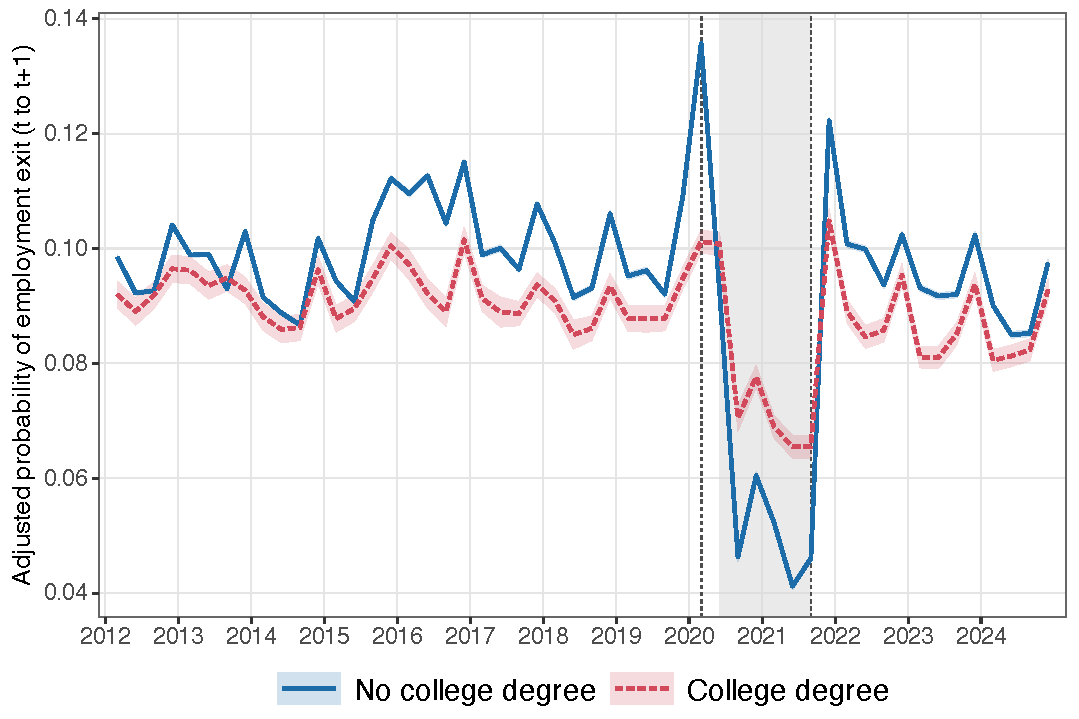
\includegraphics[width=\linewidth]{fig_levels.pdf}
  \caption{Adjusted probability of employment exit by education,
  \QfirstLab--\QlastLab. Survey-weighted average predictive margins from
  equation~\eqref{eq:es}, with 95\% pointwise bands. The shaded band marks
  2020Q2--2021Q3; the dashed lines mark 2020Q1 and 2021Q3.}
  \label{fig:levels}
\end{figure}

Three phases stand out. Through 2012--2019 the gradient is stable and runs the
expected way: the adjusted gap averages \PreGap{} (s.e.\ \PreGapSE), so
graduates are about \PreGapAbsPP{} percentage points less likely to leave
employment than otherwise comparable non-graduates. At the onset, in 2020Q1, the
gradient widens sharply to \GapOnsetQ: the first wave of exits fell
disproportionately on workers without a degree, raising their adjusted exit
level by \OnsetRelNoCol\% relative to its pre-pandemic average against
\OnsetRelCol\% for graduates. This contrast, however, is identified from a
single quarter. Its asymptotic standard error is small under every clustering
scheme in Table~\ref{tab:vcov}, including clustering on year-quarter alone, but
that is exactly the configuration in which the cluster-robust variance is known
to be badly downward biased: the deviation is picked up in one cluster out of
\Nquarters{} \citep{Cameron2008, Roodman2019}. Imposing the null and
resampling signs across quarters, the wild cluster bootstrap returns
$p=\WcbOnset$ (Table~\ref{tab:spec_ladder}). Put plainly, a movement of this
size in the education gap in a single quarter is not unusual once quarterly
shocks to the gap are taken seriously. We report the onset estimate as a
description of what happened in 2020Q1 and build nothing on it.

\begin{table}[H]
\centering
\caption{Adjusted employment-exit probabilities and the college gap, by destination and period}
\label{tab:main_margins}
\begin{threeparttable}
\footnotesize
\renewcommand{\arraystretch}{0.96}
\setlength{\tabcolsep}{4pt}
\begin{tabular}{lccccrr}
\toprule
& \multicolumn{2}{c}{Adjusted level} & \multicolumn{3}{c}{College $-$ no college} & \\
\cmidrule(lr){2-3}\cmidrule(lr){4-6}
& No college & College & Difference & 95\% CI & \multicolumn{2}{c}{\% change vs.\ pre-pandemic} \\
\cmidrule(lr){6-7}
Period & (1) & (2) & (3) & (4) & No college & College \\
\midrule
\multicolumn{7}{l}{\textit{Panel A. Employment exit}} \\
\quad Pre-pandemic & 0.099 & 0.092 & -0.008$^{***}$ & [-0.010, -0.005] & -- & -- \\
 & (0.0002) & (0.0011) & (0.0013) & & & \\
\quad Onset & 0.135 & 0.101 & -0.034$^{***}$ & [-0.037, -0.032] & 36.1 & 10.3 \\
 & (0.0003) & (0.0010) & (0.0013) & & & \\
\quad Mid-pandemic & 0.056 & 0.075 & 0.019$^{***}$ & [0.016, 0.021] & -43.5 & -18.3 \\
 & (0.0003) & (0.0010) & (0.0013) & & & \\
\quad Post-pandemic & 0.097 & 0.088 & -0.009$^{***}$ & [-0.012, -0.007] & -2.5 & -4.4 \\
 & (0.0003) & (0.0010) & (0.0013) & & & \\
\addlinespace
\multicolumn{7}{l}{\textit{Panel B. Exit into unemployment}} \\
\quad Pre-pandemic & 0.031 & 0.029 & -0.002$^{***}$ & [-0.003, -0.001] & -- & -- \\
 & (0.0001) & (0.0005) & (0.0007) & & & \\
\quad Onset & 0.040 & 0.029 & -0.011$^{***}$ & [-0.012, -0.010] & 28.2 & -0.3 \\
 & (0.0002) & (0.0005) & (0.0007) & & & \\
\quad Mid-pandemic & 0.023 & 0.024 & 0.002$^{**}$ & [0.000, 0.003] & -28.0 & -17.6 \\
 & (0.0002) & (0.0005) & (0.0006) & & & \\
\quad Post-pandemic & 0.026 & 0.026 & 0.000 & [-0.001, 0.002] & -17.0 & -9.8 \\
 & (0.0001) & (0.0005) & (0.0006) & & & \\
\addlinespace
\multicolumn{7}{l}{\textit{Panel C. Exit into non-participation}} \\
\quad Pre-pandemic & 0.068 & 0.062 & -0.006$^{***}$ & [-0.008, -0.004] & -- & -- \\
 & (0.0002) & (0.0008) & (0.0010) & & & \\
\quad Onset & 0.095 & 0.072 & -0.023$^{***}$ & [-0.026, -0.021] & 39.8 & 15.3 \\
 & (0.0002) & (0.0008) & (0.0011) & & & \\
\quad Mid-pandemic & 0.034 & 0.051 & 0.017$^{***}$ & [0.015, 0.019] & -50.6 & -18.6 \\
 & (0.0003) & (0.0008) & (0.0010) & & & \\
\quad Post-pandemic & 0.071 & 0.061 & -0.010$^{***}$ & [-0.012, -0.008] & 4.2 & -1.8 \\
 & (0.0002) & (0.0007) & (0.0010) & & & \\
\bottomrule
\end{tabular}
\begin{tablenotes}[flushleft]\scriptsize
\item Notes: Entries in columns (1)--(3) are survey-weighted average predictive margins from the event-study specification of equation~(\ref{eq:es}), which includes year-quarter, state, urban, gender, race, tenure, occupation and sector fixed effects and controls for age, age squared, usual weekly hours, log labour income, formality, temporary status and social security contribution. Margins are computed by holding the covariate distribution fixed and setting the college indicator to zero and to one in turn; they are not regression intercepts. Panel A is any exit from employment; Panels B and C split it by destination, so B and C sum to A by construction. Standard errors in parentheses are two-way clustered by primary sampling unit and year-quarter. Stars on the difference in column (3) denote $^{*}p<0.10$, $^{**}p<0.05$, $^{***}p<0.01$; the adjusted levels are probabilities and carry none. The last two columns report the percentage change in each group's adjusted level relative to its own pre-pandemic average.
\end{tablenotes}
\end{threeparttable}
\end{table}


From 2020Q2 the gradient inverts. Over the six quarters to 2021Q3 the adjusted
gap averages \MidGap{} (s.e.\ \MidGapSE, 95\% CI [\MidGapLo, \MidGapHi]),
peaking at \GapMaxRev{} in \GapMaxRevQ. The sign flips in
\NRevQuarters{} of the \Nquarters{} quarters, the six inside the window plus
\RevFirst, and the simultaneous band excludes zero in \NRevSimQuarters{} of
them, all inside the window, so this is not an artefact of testing
\Nquarters{} contrasts one at a time. Mechanically the inversion comes from
both sides: the adjusted exit level of non-graduates falls \MidRelNoColAbs\%
below its pre-pandemic average while that of graduates falls only
\MidRelColAbs\%. From 2021Q4 the pre-pandemic configuration returns, and by the end
of the sample the adjusted gap is \PostGap.

\begin{figure}[H]
  \centering
  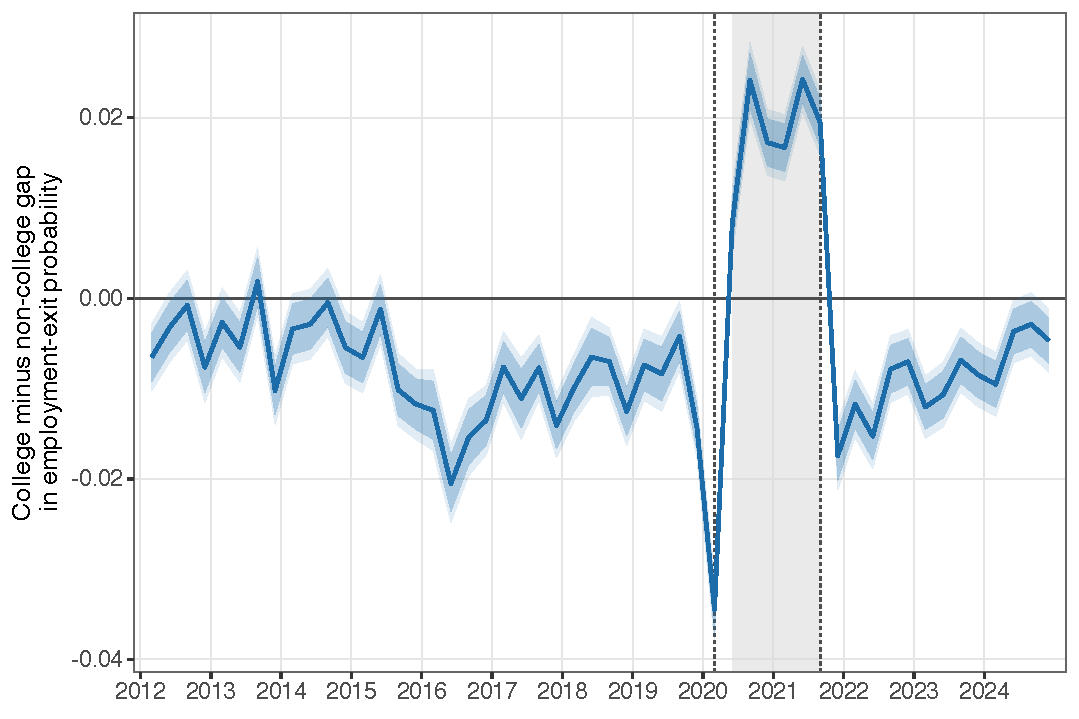
\includegraphics[width=\linewidth]{fig_gap.pdf}
  \caption{College minus non-college difference in the adjusted probability of
  employment exit. The dark band is the pointwise 95\% interval; the light band
  is the sup-$t$ simultaneous band over all \Nquarters{} quarterly contrasts
  (critical value \SuptCrit).}
  \label{fig:gap}
\end{figure}

Table~\ref{tab:spec_ladder} shows how the two pandemic contrasts move as
controls and fixed effects are added, and reports wild cluster bootstrap
$p$-values clustered by year-quarter for the preferred specification. Two
readings follow. Substantively, the reversal appears only in columns (5) and
(6): with quarter, state and demographic controls alone the mid-pandemic gap is
still negative, and it turns positive once time-varying job characteristics and
occupation and sector fixed effects are added. This is the same message the
decomposition delivers in Section~\ref{sec:decomposition}. Statistically, the
mid-pandemic contrast is unambiguous under the year-quarter bootstrap
($p\,\WcbMid$) while the onset contrast is not ($p=\WcbOnset$), for the reason
just given: one treated quarter cannot be separated from a quarterly shock.

\begin{table}[H]
\centering
\caption{The college gap in employment exits across specifications}
\label{tab:spec_ladder}
\begin{threeparttable}
\small
\setlength{\tabcolsep}{4pt}
\begin{tabular}{lcccccc}
\toprule
& (1) & (2) & (3) & (4) & (5) & (6) \\
\midrule
College, other quarters ($\delta$) & -0.069$^{***}$ & -0.069$^{***}$ & -0.060$^{***}$ & -0.053$^{***}$ & -0.023$^{***}$ & -0.010$^{***}$ \\
 & (0.001) & (0.001) & (0.001) & (0.001) & (0.001) & (0.001) \\
\addlinespace
College $\times$ onset ($\omega_1$) & -0.021$^{***}$ & -0.021$^{***}$ & -0.023$^{***}$ & -0.025$^{***}$ & -0.025$^{***}$ & -0.026 \\
 & (0.001) & (0.001) & (0.001) & (0.001) & (0.001) & (0.001) \\
\quad Wild cluster bootstrap $p$ & -- & -- & -- & -- & -- & 0.177 \\
\addlinespace
College $\times$ mid-pandemic ($\omega_2$) & 0.029$^{***}$ & 0.029$^{***}$ & 0.029$^{***}$ & 0.027$^{***}$ & 0.027$^{***}$ & 0.027$^{***}$ \\
 & (0.002) & (0.002) & (0.002) & (0.002) & (0.002) & (0.002) \\
\quad Wild cluster bootstrap $p$ & -- & -- & -- & -- & -- & $<$0.0001 \\
\midrule
\multicolumn{7}{l}{\textit{Implied college gap}} \\
\quad Onset ($\delta+\omega_1$) & -0.090$^{***}$ & -0.090$^{***}$ & -0.083$^{***}$ & -0.077$^{***}$ & -0.048$^{***}$ & -0.035$^{***}$ \\
 & (0.000) & (0.000) & (0.000) & (0.000) & (0.001) & (0.001) \\
\addlinespace
\quad Mid-pandemic ($\delta+\omega_2$) & -0.040$^{***}$ & -0.040$^{***}$ & -0.030$^{***}$ & -0.026$^{***}$ & 0.005$^{**}$ & 0.018$^{***}$ \\
 & (0.002) & (0.002) & (0.002) & (0.002) & (0.002) & (0.002) \\
\midrule
Year-quarter FE & -- & Yes & Yes & Yes & Yes & Yes \\
State and urban FE & -- & -- & Yes & Yes & Yes & Yes \\
Gender and race FE & -- & -- & -- & Yes & Yes & Yes \\
Tenure FE & -- & -- & -- & -- & Yes & Yes \\
Occupation and sector FE & -- & -- & -- & -- & -- & Yes \\
Time-varying job controls & -- & -- & -- & -- & Yes & Yes \\
\addlinespace
Observations & 8,002,128 & 8,002,128 & 8,002,128 & 8,002,128 & 8,002,128 & 8,002,128 \\
$R^2$ & 0.010 & 0.011 & 0.020 & 0.045 & 0.091 & 0.093 \\
\bottomrule
\end{tabular}
\begin{tablenotes}[flushleft]\footnotesize
\item Notes: Survey-weighted linear probability models. The dependent variable is an indicator for exiting employment between $t$ and $t+1$. $\delta$ is the college gap outside the two pandemic windows; $\omega_1$ and $\omega_2$ shift it at the onset and during the mid-pandemic window. Standard errors in parentheses are two-way clustered by primary sampling unit and year-quarter. For the two pandemic deviations we also report, for the preferred specification in column (6), wild cluster bootstrap $p$-values clustered by year-quarter (52 clusters), using Rademacher weights with the null imposed and 9,999 replications; they test $\omega_1$ and $\omega_2$, the shifts in the gap, which is where the number of quarterly shocks rather than the number of records determines uncertainty. Stars denote $^{*}p<0.10$, $^{**}p<0.05$, $^{***}p<0.01$; they are based on the wild cluster bootstrap $p$-value wherever one is reported, and on the asymptotic two-way clustered standard error otherwise. The onset deviation $\omega_1$ therefore carries no stars in column (6): identified from a single year-quarter, it cannot be told apart from an ordinary quarterly shock. The implied gaps keep their asymptotic stars because they are dominated by $\delta$, which is identified across all 52 quarters. Periods are pre-pandemic 2012Q1--2019Q4, onset 2020Q1, mid-pandemic 2020Q2--2021Q3 and post-pandemic 2021Q4--2024Q4.
\end{tablenotes}
\end{threeparttable}
\end{table}


\subsection{Where the reversal happens}\label{sec:where}

Figure~\ref{fig:formal} splits the sample by formality.

\begin{figure}[H]
  \centering
  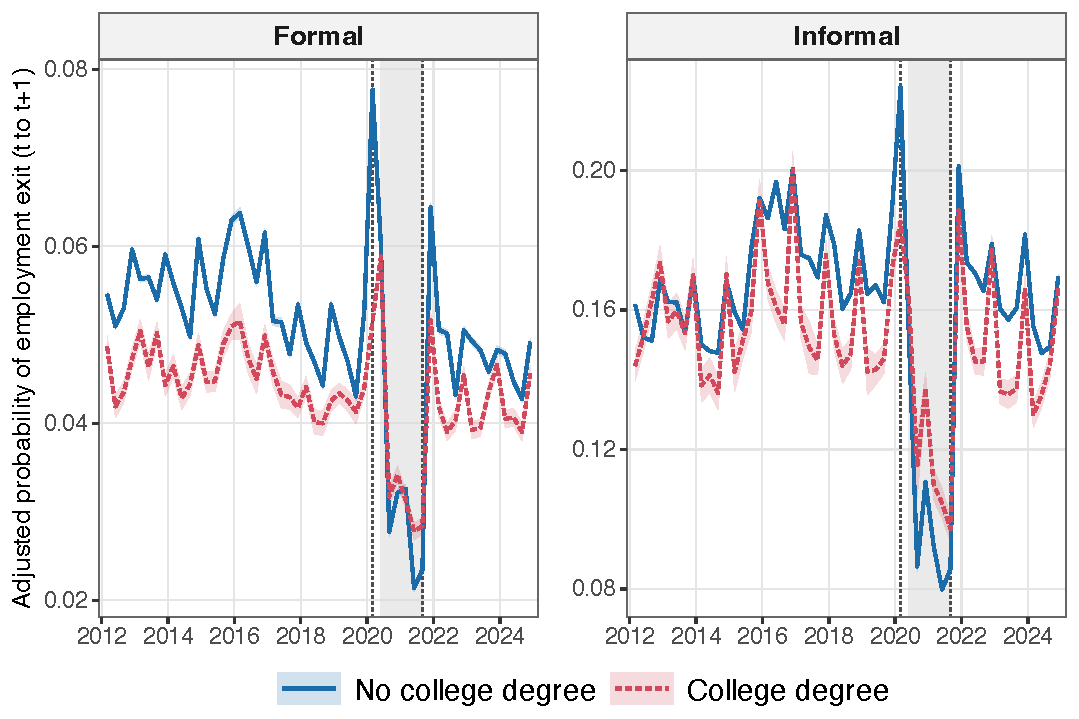
\includegraphics[width=\linewidth]{fig_formal_informal.pdf}
  \caption{Adjusted probability of employment exit by education, formal and
  informal employment estimated separately. Note the different vertical scales.}
  \label{fig:formal}
\end{figure}

Exit risk is far higher in informal employment throughout, and the reversal is
an informal-sector phenomenon. Among informal workers the adjusted gap moves
from \InformalPreGap{} before the pandemic to \InformalMidGap{} (s.e.\
\InformalMidGapSE) in 2020Q2--2021Q3. Among formal workers it moves from
\FormalPreGap{} to \FormalMidGap. The detailed position categories locate it more precisely still. The reversal is
driven by informal private employees, workers in a dependent employment
relationship without a signed work card, whose adjusted gap moves from
\InfPrivPreGap{} to \InfPrivMidGap. It is absent among the informal
self-employed (\InfSelfMidGap), among formal private employees
(\FormPrivMidGap) and among formal public servants (\FormPubMidGap); only the
formal self-employed show a smaller echo of it (\FormSelfMidGap).
Figure~\ref{fig:position} shows the four groups separately, and
Table~\ref{tab:heterogeneity} reports all segments.

\begin{figure}[H]
  \centering
  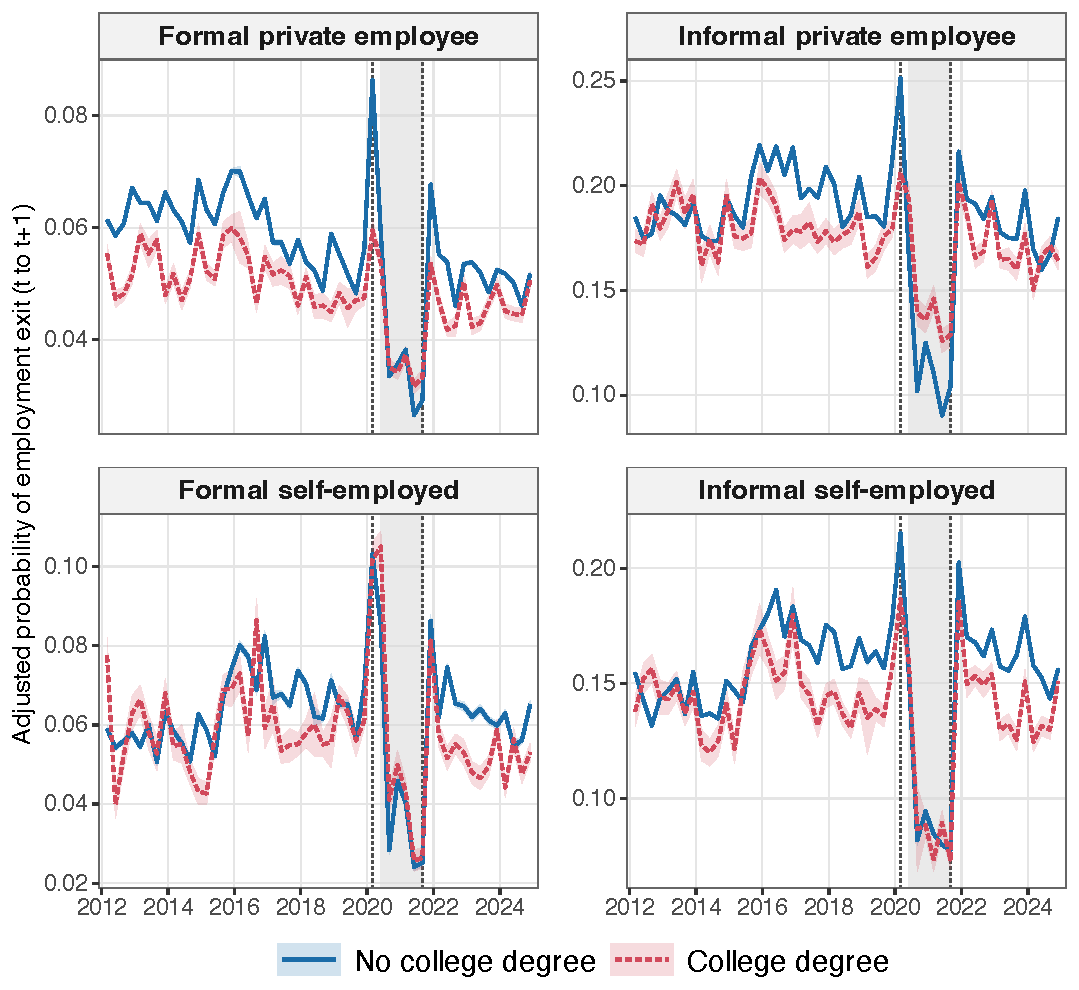
\includegraphics[width=\linewidth]{fig_by_position.pdf}
  \caption{Adjusted probability of employment exit by education and labour
  market position. Each panel is estimated on its own subsample; public-sector
  employees are reported separately in Table~\ref{tab:heterogeneity}. Note the
  different vertical scales.}
  \label{fig:position}
\end{figure}

That the movement is concentrated among informal employees rather than
the informal self-employed is informative. Dismissal risk is the margin that
moves, and it moves for the unprotected wage workers whose separations are
employer decisions, not for own-account workers whose exits are largely their
own. It also means the pattern cannot be read as a pure labour-supply response
to the transfer, which would have been at least as visible among the
self-employed.

\begin{table}[H]
\centering
\caption{Adjusted college gap in employment exits, by labour market segment}
\label{tab:heterogeneity}
\begin{threeparttable}
\small
\setlength{\tabcolsep}{4pt}
\begin{tabular}{lccccr}
\toprule
Segment & Pre-pandemic & Onset & Mid-pandemic & Post-pandemic & Obs. \\
\midrule
\addlinespace\multicolumn{6}{l}{\textit{Formality}} \\
\quad Formal & -0.009$^{***}$ & -0.026$^{***}$ & 0.002$^{***}$ & -0.006$^{***}$ & 4,363,453 \\
 & (0.001) & (0.001) & (0.001) & (0.001) & \\
\quad Informal & -0.014$^{***}$ & -0.040$^{***}$ & 0.019$^{***}$ & -0.019$^{***}$ & 3,638,675 \\
 & (0.002) & (0.003) & (0.002) & (0.002) & \\
\addlinespace\multicolumn{6}{l}{\textit{Gender}} \\
\quad Men & -0.004$^{***}$ & -0.029$^{***}$ & 0.015$^{***}$ & -0.005$^{***}$ & 4,656,560 \\
 & (0.001) & (0.001) & (0.001) & (0.001) & \\
\quad Women & -0.013$^{***}$ & -0.043$^{***}$ & 0.025$^{***}$ & -0.016$^{***}$ & 3,345,568 \\
 & (0.002) & (0.002) & (0.002) & (0.002) & \\
\addlinespace\multicolumn{6}{l}{\textit{Position}} \\
\quad Formal private employee & -0.009$^{***}$ & -0.027$^{***}$ & 0.000 & -0.006$^{***}$ & 2,679,329 \\
 & (0.001) & (0.001) & (0.001) & (0.001) & \\
\quad Formal public sector & -0.004$^{***}$ & -0.007$^{***}$ & -0.003$^{***}$ & -0.007$^{***}$ & 818,008 \\
 & (0.001) & (0.001) & (0.001) & (0.001) & \\
\quad Formal self-employed & -0.005$^{***}$ & -0.003 & 0.008$^{***}$ & -0.011$^{***}$ & 624,666 \\
 & (0.002) & (0.003) & (0.002) & (0.001) & \\
\quad Informal private employee & -0.015$^{***}$ & -0.045$^{***}$ & 0.029$^{***}$ & -0.015$^{***}$ & 1,674,121 \\
 & (0.002) & (0.004) & (0.003) & (0.002) & \\
\quad Informal self-employed & -0.014$^{***}$ & -0.027$^{***}$ & -0.001 & -0.022$^{***}$ & 1,621,692 \\
 & (0.002) & (0.004) & (0.003) & (0.002) & \\
\addlinespace\multicolumn{6}{l}{\textit{Race}} \\
\quad Non-White & -0.013$^{***}$ & -0.032$^{***}$ & 0.022$^{***}$ & -0.013$^{***}$ & 4,582,254 \\
 & (0.001) & (0.002) & (0.002) & (0.001) & \\
\quad White & -0.009$^{***}$ & -0.034$^{***}$ & 0.010$^{***}$ & -0.009$^{***}$ & 3,419,874 \\
 & (0.001) & (0.001) & (0.001) & (0.001) & \\
\bottomrule
\end{tabular}
\begin{tablenotes}[flushleft]\footnotesize
\item Notes: Each cell is the survey-weighted average predictive difference in the probability of exiting employment between workers with and without a college degree, estimated on the indicated subsample with the full specification of equation~(\ref{eq:es}). Fixed effects and controls that are collinear within a segment are dropped. Standard errors in parentheses are two-way clustered by primary sampling unit and year-quarter. Stars denote $^{*}p<0.10$, $^{**}p<0.05$, $^{***}p<0.01$. Periods are pre-pandemic 2012Q1--2019Q4, onset 2020Q1, mid-pandemic 2020Q2--2021Q3 and post-pandemic 2021Q4--2024Q4.
\end{tablenotes}
\end{threeparttable}
\end{table}


\subsection{Composition or within-cell risk?}\label{sec:decomposition}

The decomposition in equation~\eqref{eq:decomp} separates the two explanations.
Figure~\ref{fig:decomp} plots the components quarter by quarter and
Table~\ref{tab:decomposition} reports period averages.

\begin{figure}[H]
  \centering
  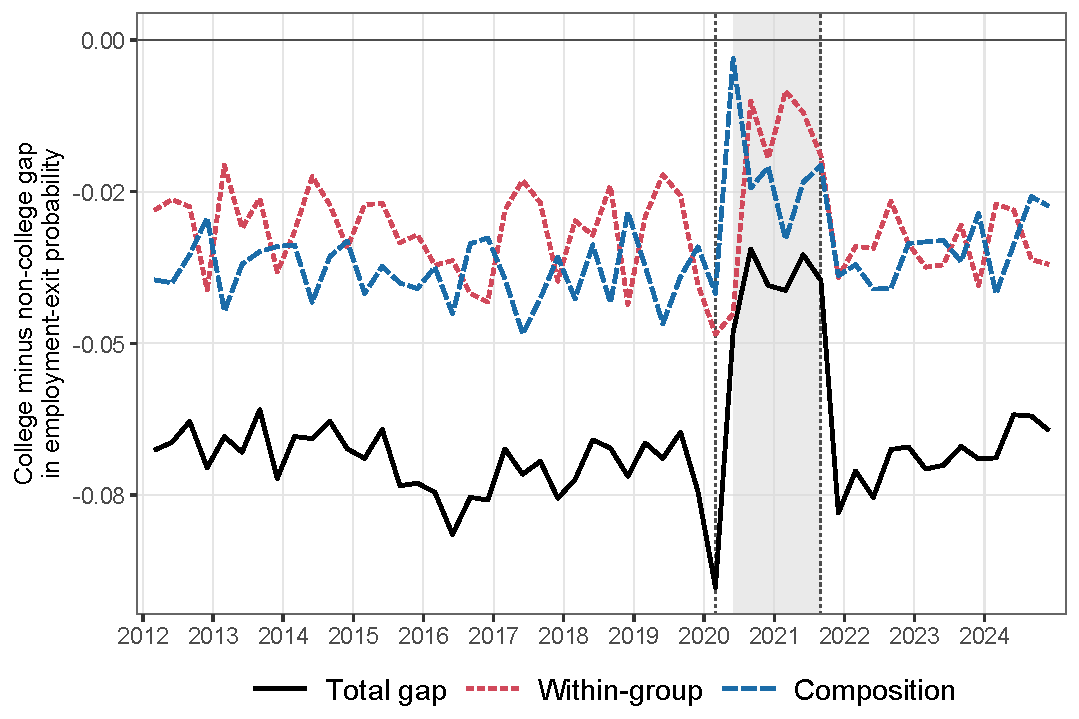
\includegraphics[width=\linewidth]{fig_decomposition.pdf}
  \caption{Composition and within-cell components of the raw education gap in
  employment exits. Cells are defined by formality $\times$ sector $\times$
  occupation.}
  \label{fig:decomp}
\end{figure}

Two things stand out, and both hold under either cell definition. First, neither
margin dominates. Composition accounts for \DecPreCompShare\% of the raw
pre-pandemic gap (\DecPreComp{} out of \DecPreTotal) and within-cell risk for
the remaining \DecPreWithinShare\% (\DecPreWithin), and those shares are
essentially unchanged in every other period. Graduates are safer partly because
they hold formal jobs in more protected occupations and sectors, and partly
because they are safer inside those jobs.

Second, and more informative, the two components compress together
during 2020Q2--2021Q3: composition by \DecCompShrink\% and within-cell risk by
\DecWithinShrink\%. The raw gap therefore halves, from \DecPreTotal{} to
\DecMidTotal, without changing sign, and the split between the two channels is
the same before, during and after. The mid-pandemic narrowing is not a
reallocation story: graduates did not move into riskier cells.

This locates the reversal of Figure~\ref{fig:gap} precisely. It is not visible
at the level of formality, sector and occupation, where the education advantage
merely shrinks by about half. It emerges only once the richer conditioning set
of equation~\eqref{eq:es} is applied, that is, once two workers are matched not
only on cell but also on hours, labour income, tenure, contract type, social
security status and location. Inside a given formality-sector-occupation cell,
graduates still hold the better-paid, longer-tenured, contractually protected
jobs. Strip that residual advantage away as well and, for six quarters, their
edge in staying employed does not merely disappear: it turns negative.

\begin{table}[H]
\centering
\caption{Composition versus within-cell decomposition of the education gap}
\label{tab:decomposition}
\begin{threeparttable}
\begin{tabular}{lcccc}
\toprule
& Total gap & Composition & Within-cell & Within-cell \\
Period & $\Delta^{\mathrm{raw}}_q$ & component & component & share (\%) \\
\midrule
\multicolumn{5}{l}{\textit{Cells: formality $\times$ sector $\times$ occupation (100 cells)}} \\
\quad Pre-pandemic & -0.069$^{***}$ & -0.038$^{***}$ & -0.031$^{***}$ & 44.9 \\
 & & [-0.041, -0.035] & [-0.034, -0.028] & \\
\quad Onset & -0.090 & -0.042 & -0.048 & 53.7 \\
\quad Mid-pandemic & -0.040$^{***}$ & -0.021$^{***}$ & -0.019$^{***}$ & 47.5 \\
 & & [-0.029, -0.010] & [-0.033, -0.009] & \\
\quad Post-pandemic & -0.069$^{***}$ & -0.035$^{***}$ & -0.034$^{***}$ & 49.5 \\
 & & [-0.039, -0.030] & [-0.038, -0.029] & \\
\addlinespace
\multicolumn{5}{l}{\textit{Cells: formality $\times$ position $\times$ sector $\times$ occupation (382 cells)}} \\
\quad Pre-pandemic & -0.069$^{***}$ & -0.042$^{***}$ & -0.028$^{***}$ & 39.8 \\
 & & [-0.044, -0.039] & [-0.031, -0.024] & \\
\quad Onset & -0.090 & -0.052 & -0.038 & 42.2 \\
\quad Mid-pandemic & -0.040$^{***}$ & -0.024$^{***}$ & -0.016$^{***}$ & 40.6 \\
 & & [-0.031, -0.014] & [-0.029, -0.007] & \\
\quad Post-pandemic & -0.069$^{***}$ & -0.037$^{***}$ & -0.031$^{***}$ & 45.3 \\
 & & [-0.043, -0.033] & [-0.036, -0.026] & \\
\bottomrule
\end{tabular}
\begin{tablenotes}[flushleft]\footnotesize
\item Notes: The total gap is the survey-weighted difference in the raw employment-exit rate between workers with and without a college degree. The composition component holds each cell's non-college exit rate fixed and varies only the two groups' allocation across cells; the within-cell component holds the college allocation fixed and varies only the exit rates inside cells. Period figures are averages of the quarterly components weighted by the quarter's share of the total survey weight. A cell is a combination of the listed variables that some worker occupies: formality is the two-way formal / informal split, sector the five broad activity groups, occupation the ten COD major groups and position the eight labour-market categories of Table~\ref{tab:heterogeneity} (private employee, self-employed, employer and public sector, each formal or informal). The cell counts are the combinations actually observed; the remaining 32 and 212 combinations the crossings allow are empty. Cells occupied by only one education group hold 0.2% and 0.6% of the survey weight under the two definitions; they have no counterfactual rate for the absent group, so their whole contribution falls on the within-cell component. Brackets report 95\% percentile intervals from 2000 replications of a two-way pigeonhole bootstrap that resamples primary sampling units and quarters independently. Stars denote $^{*}p<0.10$, $^{**}p<0.05$, $^{***}p<0.01$ on the bootstrap standard error of the entry. The onset is a single quarter, for which a bootstrap over quarters carries no information, so it is reported without an interval. Periods are pre-pandemic 2012Q1--2019Q4, onset 2020Q1, mid-pandemic 2020Q2--2021Q3 and post-pandemic 2021Q4--2024Q4.
\end{tablenotes}
\end{threeparttable}
\end{table}


\subsection{Gender and race}

Table~\ref{tab:heterogeneity} and Figure~\ref{fig:demographics} report the
same adjusted margins by gender and by race. The pre-pandemic gradient is not uniform:
it is markedly steeper for women (\WomenPreGap) than for men (\MenPreGap), and
steeper for non-white workers (\NonWhitePreGap) than for white workers
(\WhitePreGap). The mid-pandemic reversal nonetheless appears in every group,
at \MenMidGap{} for men and \WomenMidGap{} for women, and \WhiteMidGap{} for
white and \NonWhiteMidGap{} for non-white workers. It is therefore not a composition artefact of one
demographic group driving the aggregate. Its magnitude, however, tracks
informality: it is largest among women and among non-white workers, the two
groups whose employment is most concentrated in the informal segment, which is
what the reading in Section~\ref{sec:where} implies.

\begin{figure}[H]
  \centering
  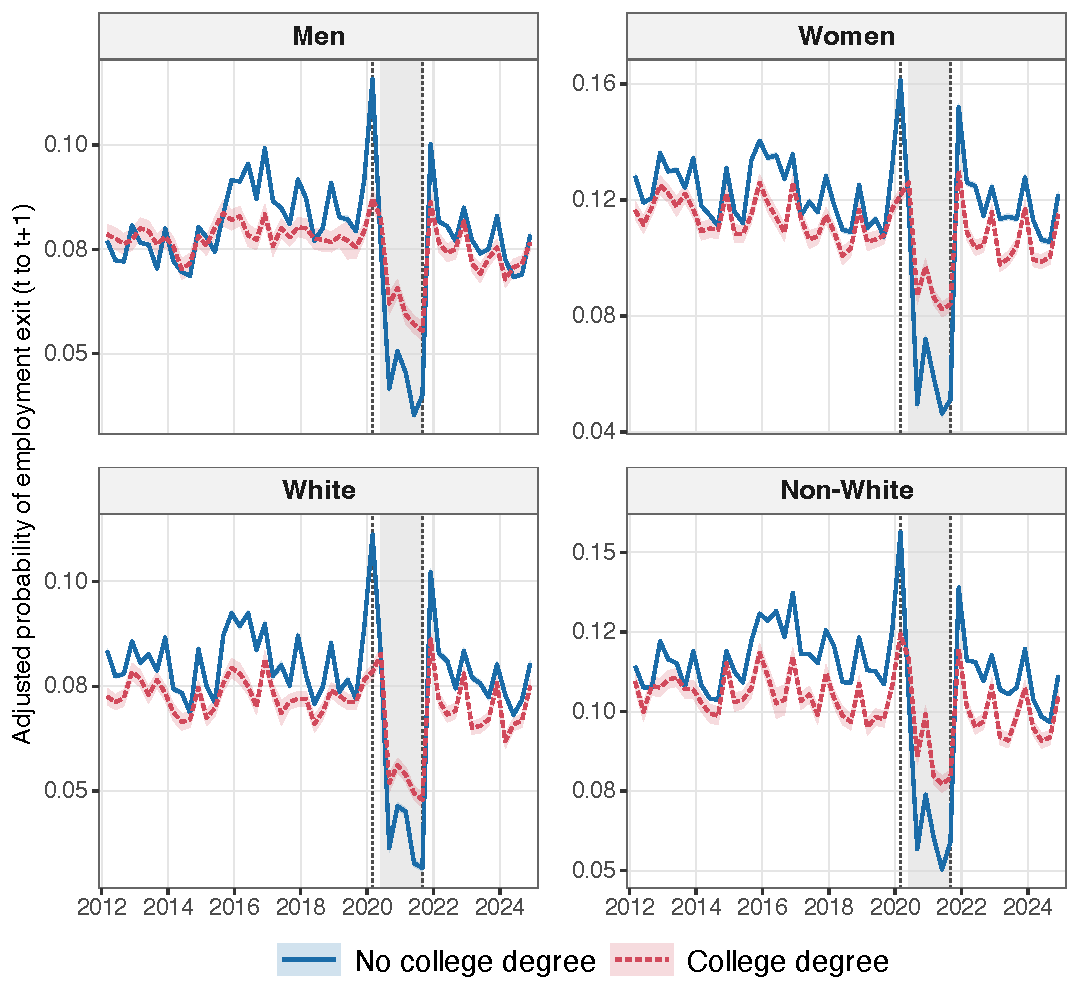
\includegraphics[width=\linewidth]{fig_by_demographics.pdf}
  \caption{Adjusted probability of employment exit by education, within
  demographic groups. Each panel is estimated on its own subsample, with 95\%
  pointwise bands. Note the different vertical scales.}
  \label{fig:demographics}
\end{figure}

%==============================================================================
\section{Panel retention and selection}\label{sec:attrition}
%==============================================================================

The outcome exists only for workers the matching algorithm finds again, so
differential retention is a first-order concern: if graduates and non-graduates
became differentially harder to re-interview in 2020--2021, part of the reversal
could be an artefact.

The selection that generates the estimation sample is the match from $t$ into
$t+1$, and here it is observed directly. The build keeps every worker employed
in quarter $t$, whether or not the algorithm finds them again, so the indicator
we model is the very object at issue rather than a stand-in for it.

One restriction applies. A household is interviewed five consecutive quarters,
so a worker observed in the fifth interview has no $t+1$ inside the panel: that
is a scheduled exit, not attrition. The survey's own interview counter
identifies those rows exactly, and we drop them. Figure~\ref{fig:retention}
plots the resulting match rate and Table~\ref{tab:attrition} summarises.

\begin{figure}[H]
  \centering
  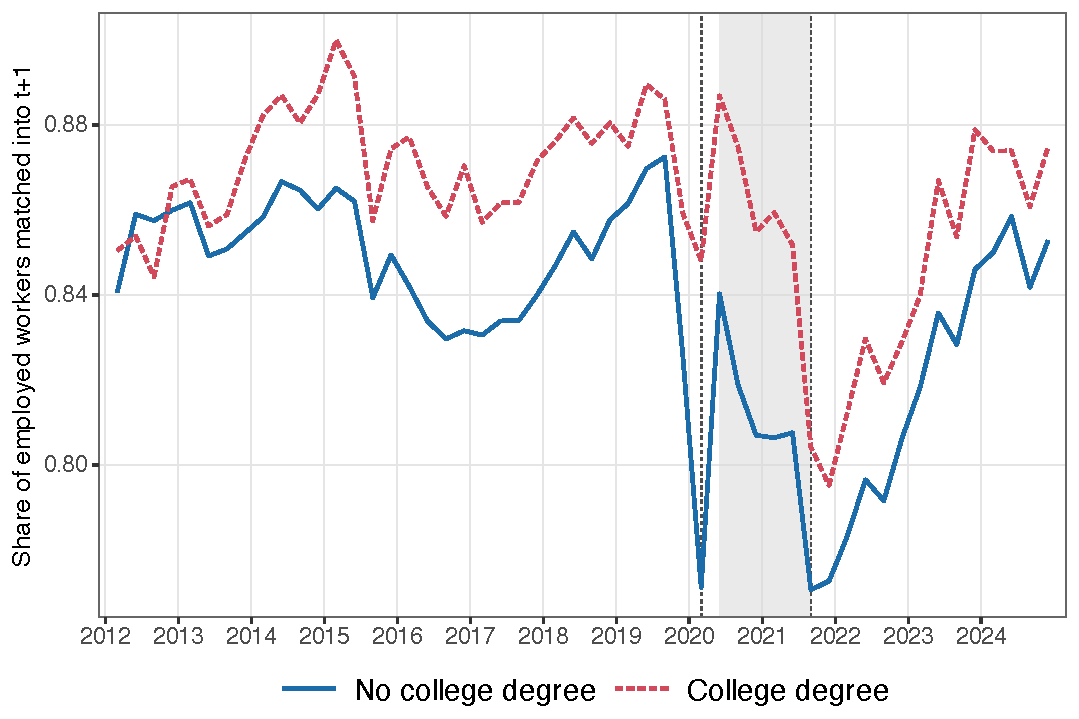
\includegraphics[width=\linewidth]{fig_retention.pdf}
  \caption{Share of employed workers matched into the following quarter, by
  education. Sample restricted to interviews 1--4, the interviews for which a
  further one is scheduled.}
  \label{fig:retention}
\end{figure}

Graduates are consistently easier to re-find, and the pandemic widened the gap.
The college / non-college difference in the match rate is \RetDiffPre{} before
the pandemic, jumps to \RetDiffOnset{} in 2020Q1 when fieldwork switched to
telephone interviewing, and is still \RetDiffMid{} through 2020Q2--2021Q3
before settling back. This is exactly the pattern that should make a reader
uneasy: the workers we lose track of are disproportionately non-graduates, and
we lose more of them precisely in the quarters where the gradient moves. Panel B
of Table~\ref{tab:attrition} shows the same thing in levels, with the largest
standardised differences on formality and labour income.

Two things bound the concern. The first is the re-weighting below, which prices
in the differential directly and barely moves the estimate. The second is that
selective attrition of this kind pushes the mid-pandemic gap in the wrong
direction to explain it: the workers dropping out of view are the ones with the
higher exit risk, so their absence understates non-graduate exits and therefore
understates, rather than manufactures, a reversal in which graduates exit
more.

\begin{table}[H]
\centering
\caption{Panel retention and selection into the matched sample}
\label{tab:attrition}
\begin{threeparttable}
\begin{tabular}{lcccccc}
\multicolumn{7}{l}{\textit{Panel A. Share of employed workers matched into $t+1$}} \\
\toprule
& \multicolumn{3}{c}{By education} & \multicolumn{3}{c}{By formality} \\
\cmidrule(lr){2-4}\cmidrule(lr){5-7}
Period & No college & College & Diff. & Formal & Informal & Diff. \\
\midrule
Pre-pandemic & 0.851 & 0.872 & 0.021 & 0.856 & 0.851 & 0.005 \\
Onset & 0.771 & 0.848 & 0.077 & 0.808 & 0.757 & 0.051 \\
Mid-pandemic & 0.807 & 0.855 & 0.048 & 0.827 & 0.806 & 0.021 \\
Post-pandemic & 0.822 & 0.848 & 0.026 & 0.831 & 0.824 & 0.007 \\
\bottomrule
\addlinespace
\multicolumn{7}{l}{\textit{Panel B. Matched vs.\ unmatched origins, all quarters}} \\
\toprule
& Matched & Unmatched & Std.\ diff. & & & \\
\midrule
College degree & 0.199 & 0.170 & 0.073 & & & \\
Woman & 0.428 & 0.407 & 0.042 & & & \\
Non-White & 0.534 & 0.585 & -0.102 & & & \\
Urban area & 0.875 & 0.898 & -0.071 & & & \\
Age & 39.028 & 36.476 & 0.199 & & & \\
Usual weekly hours & 39.285 & 40.001 & -0.061 & & & \\
Log labour income & 6.904 & 6.954 & -0.029 & & & \\
Formal employment & 0.603 & 0.588 & 0.030 & & & \\
Signed work card & 0.406 & 0.437 & -0.062 & & & \\
Social security contributor & 0.151 & 0.120 & 0.093 & & & \\
Temporary job & 0.072 & 0.076 & -0.014 & & & \\
\bottomrule
\end{tabular}
\begin{tablenotes}[flushleft]\footnotesize
\item Notes: The sample is every worker employed at the interview date in quarter $t$ who is not in the fifth and final interview of their household's rotation, so that a further interview is scheduled. Retention equals one when the stage-3 algorithm links the worker into $t+1$. Panel B reports survey-weighted means and the standardised difference, $(\bar{x}_1-\bar{x}_0)/\sqrt{(s_1^2+s_0^2)/2}$. Periods are pre-pandemic 2012Q1--2019Q4, onset 2020Q1, mid-pandemic 2020Q2--2021Q3 and post-pandemic 2021Q4--2024Q4.
\end{tablenotes}
\end{threeparttable}
\end{table}


We then re-weight. A separate logit per quarter, on education, demographics,
job characteristics and state, occupation and sector fixed effects, gives each
worker a predicted probability of being matched forward; fitting it quarter by
quarter lets every coefficient, not only the one on education, move over time.
Multiplying the survey weight by the inverse of that probability, trimmed at
0.05, and re-estimating equation~\eqref{eq:es} leaves the mid-pandemic gap
essentially unchanged, at \IpwMidGapFour{} against \BaseMidGapFour{} on the
same sample without re-weighting: the two agree to three decimals
(Table~\ref{tab:ipw}).

\begin{table}[htbp]
\centering
\caption{The adjusted college gap under inverse-retention-probability weighting}
\label{tab:ipw}
\begin{threeparttable}
\begin{tabular}{lcc}
\toprule
& Survey weights & Survey $\times$ inverse-retention weights \\
Period & (1) & (2) \\
\midrule
Pre-pandemic & -0.009$^{***}$ & -0.009$^{***}$ \\
 & (0.001) & (0.001) \\
Onset & -0.035$^{***}$ & -0.035$^{***}$ \\
 & (0.001) & (0.001) \\
Mid-pandemic & 0.018$^{***}$ & 0.018$^{***}$ \\
 & (0.001) & (0.001) \\
Post-pandemic & -0.010$^{***}$ & -0.010$^{***}$ \\
 & (0.001) & (0.001) \\
\bottomrule
\end{tabular}
\begin{tablenotes}[flushleft]\footnotesize
\item Notes: Both columns are estimated on the matched origins of the retention sample (8,002,128 person-quarters) with the full specification, so the two differ only in the weights. Column (2) multiplies the survey weight by the inverse of a predicted probability of being matched into $t+1$, trimmed at 0.05, from a separate logit per year-quarter on education, demographics, job characteristics and state, occupation and sector fixed effects. Standard errors are two-way clustered by primary sampling unit and year-quarter. Periods are pre-pandemic 2012Q1--2019Q4, onset 2020Q1, mid-pandemic 2020Q2--2021Q3 and post-pandemic 2021Q4--2024Q4.
\end{tablenotes}
\end{threeparttable}
\end{table}


Finally, a breakdown calculation bounds what unobserved attrition could do.
The algorithm links \MatchRateAll\% of the employed workers for whom a
further interview is scheduled into $t+1$ (Table~\ref{tab:matching}), leaving
the rest unobserved. Writing $\rho$ for that match rate, the education
gap among all such workers is
$\rho\widehat\Delta + (1-\rho)(\tilde m_C - \tilde m_N)$, where $\tilde m_g$ is
the unobserved exit rate of unmatched workers in group $g$. Setting that
expression to zero requires an unmatched-worker exit-rate differential of
$\tilde m_C - \tilde m_N = \BreakdownMid$, opposite in sign to what is observed
among matched workers and several times larger in magnitude. We regard that as
implausible, though not impossible.

%==============================================================================
\section{Robustness}\label{sec:robustness}
%==============================================================================

Table~\ref{tab:robustness} collects the remaining checks. Restricting to
prime-age workers aged 25--54 removes retirement and schooling transitions from
the outcome and leaves the pattern intact. Dropping the survey weights, and
moving the base quarter to 2019Q1, do the same. Replacing the outcome by an
indicator for being informally employed in $t+1$ shows the complementary margin
of adjustment. There the education gradient runs the usual way throughout and
widens during the window, from \PreGapInf{} to \MidGapInf: graduates
who kept working became relatively less exposed to informal employment at
exactly the time when their advantage in staying employed at all disappeared.
Table~\ref{tab:vcov} shows that the two pandemic contrasts are robust to the
choice of variance estimator, including clustering on year-quarter alone, which
is the most conservative option available given \Nquarters{} clusters.

\begin{table}[H]
\centering
\caption{Robustness of the adjusted college gap}
\label{tab:robustness}
\begin{threeparttable}
\small
\setlength{\tabcolsep}{4pt}
\begin{tabular}{lccccr}
\toprule
Specification & Pre-pandemic & Onset & Mid-pandemic & Post-pandemic & Obs. \\
\midrule
Baseline & -0.009$^{***}$ & -0.035$^{***}$ & 0.018$^{***}$ & -0.010$^{***}$ & 8,002,128 \\
 & (0.001) & (0.001) & (0.001) & (0.001) & \\
Prime age 25--54 & -0.008$^{***}$ & -0.037$^{***}$ & 0.009$^{***}$ & -0.012$^{***}$ & 5,570,238 \\
 & (0.001) & (0.001) & (0.001) & (0.001) & \\
Unweighted & -0.011$^{***}$ & -0.026$^{***}$ & 0.024$^{***}$ & -0.015$^{***}$ & 8,002,128 \\
 & (0.001) & (0.001) & (0.001) & (0.001) & \\
Base quarter 2019Q1 & -0.009$^{***}$ & -0.035$^{***}$ & 0.018$^{***}$ & -0.010$^{***}$ & 8,002,128 \\
 & (0.001) & (0.001) & (0.001) & (0.001) & \\
Outcome: informal employment in $t+1$ & -0.028$^{***}$ & -0.009$^{***}$ & -0.047$^{***}$ & -0.020$^{***}$ & 8,002,128 \\
 & (0.002) & (0.002) & (0.002) & (0.002) & \\
\bottomrule
\end{tabular}
\begin{tablenotes}[flushleft]\footnotesize
\item Notes: Each row reports survey-weighted average predictive differences in the outcome between workers with and without a college degree, from the full specification of equation~(\ref{eq:es}). The last row replaces the outcome by an indicator for being informally employed in $t+1$ -- a destination state, not a transition, so it includes workers who were already informal in $t$. Standard errors in parentheses are two-way clustered by primary sampling unit and year-quarter. Stars denote $^{*}p<0.10$, $^{**}p<0.05$, $^{***}p<0.01$. Periods are pre-pandemic 2012Q1--2019Q4, onset 2020Q1, mid-pandemic 2020Q2--2021Q3 and post-pandemic 2021Q4--2024Q4.
\end{tablenotes}
\end{threeparttable}
\end{table}


%==============================================================================
\section{Discussion}\label{sec:discussion}
%==============================================================================

The results say something specific. Schooling protects Brazilian workers from
employment exits through two channels of comparable size: placement into formal
jobs in more protected occupations and sectors, and a residual advantage inside
those cells. Neither dominates, and their relative weights are stable over time.
During 2020Q2--2021Q3 both compress by roughly the same proportion, halving the
raw gap without reversing it. The reversal appears only when workers are also
matched on the job characteristics that vary within cells, such as pay, hours,
tenure and contract type, and it appears in informal employment, specifically
among informal private employees.

We are correspondingly careful about the onset. Its point estimate is large, but
a single quarter carries no information that survives clustering on time, so
nothing in what follows rests on it. The timing of the reversal is consistent
with, but does not identify, a role for the emergency transfer and
employment-preservation programmes. \textit{Aux\'ilio Emergencial}
started in April 2020 and ended in October 2021, bracketing the window almost
exactly, and it reached precisely the informal, lower-education workers whose
adjusted exit risk fell most. The employment-preservation programme worked on
the formal side, where we find much smaller movements. But the design here has
no eligibility discontinuity and no pre-determined exposure measure, so we
cannot separate the programmes from everything else that moved at the same
time: sectoral shutdowns, differential remote-work feasibility
\citep{Dingel2020}, changed labour supply of graduates with children
\citep{Alon2020}, or the composition of who kept searching. The United States
experience with pandemic unemployment benefits illustrates how sharply such
programmes can alter measured transitions even when they are not designed to
\citep{Ganong2020, Marinescu2021}. Establishing the
policy channel would require variation in eligibility or in pre-determined
exposure, which we do not have. Claims that ``policy design matters'' go beyond
what this evidence supports; what it supports is that the education gradient in
job security is not a structural constant, and that it moved in the segment of
the labour market where the segmented policy response was concentrated.

One limitation remains. The design is descriptive. We observe that the
gradient reversed in informal wage employment during exactly the window in which
the emergency transfer operated, but we do not observe anyone who was ineligible
for it. Nothing here rules out a coincident shock with the same timing and the
same incidence.

The transferable lesson is about the architecture of emergency support rather
than about Brazil. When protection is delivered through
two channels that are segmented along the formal--informal margin, and when
schooling predicts which channel a worker falls into, the aggregate relationship
between education and job security can temporarily detach. Any country with a
large informal sector and a bifurcated safety net has the same structure.

%==============================================================================
\section{Conclusion}\label{sec:conclusion}
%==============================================================================

Using \Nobs{} matched person-quarters from \textit{PNAD Cont\'inua} over
\QfirstLab--\QlastLab, we document that Brazil's education gradient in
employment exits reversed for six quarters between 2020Q2 and 2021Q3 and then
returned to its pre-pandemic configuration. The single-quarter widening at the
onset, though large in point estimate, does not survive inference clustered on
time and we do not build on it. The reversal is present in adjusted margins computed with
design-based clustering and simultaneous bands, runs entirely through exits out
of the labour force rather than into measured unemployment, is concentrated in
informal wage employment, and survives weighting by the inverse probability of
being matched into the following quarter. A composition / within-cell
decomposition shows that the education advantage divides about evenly between
where graduates work and how they fare inside those jobs, and that both halves
compressed by roughly \DecWithinShrink\% during the window in which Brazil's
emergency transfer was operating, so the reversal is a statement about workers
matched on job characteristics, not about reallocation across sectors. The episode is a reminder that the protective value of schooling
runs through the structure of the labour market, and that policy can reshape
that structure quickly.

%==============================================================================
\section*{Declarations}
%==============================================================================

\paragraph{CRediT author statement}
\textbf{Francisco Cavalcanti:} Conceptualization, Methodology, Supervision,
Writing -- review and editing.
\textbf{Fredie Didier:} Conceptualization, Data curation, Formal analysis,
Software, Visualization, Writing -- original draft.
\textbf{Gustavo Gonzaga:} Conceptualization, Methodology, Validation,
Writing -- review and editing.

\paragraph{Declaration of competing interest}
The authors declare that they have no known competing financial interests or
personal relationships that could have appeared to influence the work reported
in this paper.

\paragraph{Declaration of generative AI use}
During the preparation of this work the authors used generative AI tools to
assist with code refactoring and language editing. The authors reviewed and
edited all output and take full responsibility for the content of the
publication.

\paragraph{Data availability}
\textit{PNAD Cont\'inua} microdata are public and distributed by \textit{IBGE}.
The rotating-panel links are built with the open-source \textit{Data Zoom}
package. All code needed to reproduce every table and figure, together with the
variable dictionary, matching rules, package versions and random seeds, is
available in the project's
\href{https://github.com/FredieDidier/Monografia}{GitHub repository}; see
\appref{app:data}.

%==============================================================================
\bibliographystyle{elsarticle-harv}
\bibliography{refs}

%==============================================================================
\appendix
%==============================================================================
% Elsevier asks for appendix tables and figures to be numbered separately, as
% Table A.1 and Fig. A.1, restarting in each appendix. \numberwithin is not
% usable here: elsarticle sets \thesection to the string "Appendix A", so it
% produces "Table Appendix A.1". The counters are therefore reset by hand at
% the start of each appendix.
\setcounter{table}{0}\renewcommand{\thetable}{A.\arabic{table}}
\setcounter{figure}{0}\renewcommand{\thefigure}{A.\arabic{figure}}
\setcounter{equation}{0}\renewcommand{\theequation}{A.\arabic{equation}}

\section{Data, matching and variable definitions}\label{app:data}

\subsection{Panel construction}

\textit{PNAD Cont\'inua} draws a master sample of census tracts and interviews
each selected household five times, once per quarter. Thirteen rotation groups
are in the field over our sample period. Data collection is spread over the
twelve weeks of the quarter.

Because no individual identifier is published, respondents have to be linked
across interviews. The first pass of the stage-3 procedure is the classical rule
of \citet{Ribas2008}, developed for the \textit{IBGE} monthly employment survey
(\textit{PME}), which matches on the household identifier together with sex and
date of birth while allowing for limited recording error. The two further passes
described in Section~\ref{sec:data} donate birth dates across a respondent's
interviews and resolve fragmented sequences with a graph-theoretic match.
Table~\ref{tab:matching} reports the performance of the procedure as a whole.

\begin{table}[H]
\centering
\caption{Performance of the stage-3 panel identification}
\label{tab:matching}
\begin{threeparttable}
\begin{tabular}{lccccc}
\multicolumn{6}{l}{\textit{Panel A. Share linked across at least $k$ interviews (\%)}} \\
\toprule
& $k=1$ & $k=2$ & $k=3$ & $k=4$ & $k=5$ \\
\midrule
Individuals & 100.0 & 84.2 & 71.7 & 60.4 & 47.1 \\
Households & 100.0 & 92.9 & 85.1 & 75.6 & 60.9 \\
\bottomrule
\addlinespace
\multicolumn{6}{l}{\textit{Panel B. Share matched into the next quarter, by interview (\%)}} \\
\toprule
& From 1st & From 2nd & From 3rd & From 4th & Overall \\
\midrule
Employed workers & 83.2 & 84.2 & 84.6 & 84.9 & 84.2 \\
\bottomrule
\end{tabular}
\begin{tablenotes}[flushleft]\footnotesize
\item Notes: Computed on all quarterly \textit{PNAD Cont\'inua} rotation panels used in the paper. Panel A covers the whole panel population and reports the share of linked units observed in at least $k$ of the five scheduled interviews. Panel B is restricted to workers employed at the interview date and reports the share the algorithm links into the following quarter, by the interview they are observed in; the fifth interview is the last scheduled one and is excluded. Stage 3 links respondents on household, sex and date of birth, donates birth dates across interviews, and resolves fragmented sequences with a fuzzy match on the date of birth that never assigns two interviews of the same quarter to one person.
\end{tablenotes}
\end{threeparttable}
\end{table}


The build in this paper reconstructs the panel from the published quarterly
microdata. Each quarter is downloaded
once, cleaned with \textit{Data Zoom}'s own routine and cached; the stage-3
identification is then run separately on each of the thirteen rotation groups.
Because a household belongs to exactly one group and the algorithm only ever
compares rows within the data it is given, running it group by group is
equivalent to running it on the whole file, while keeping peak memory bounded.
The sampling unit, the stratum and the interview counter survive the build as
ordinary columns, which is what the inference and the attrition analysis need.

\subsection{Variable definitions}

In \textit{PNAD Cont\'inua} the working-age population is aged 14 and over. A
person is employed if they worked at least one hour for pay in the
reference week, worked without pay in a family business, or were temporarily
absent from a job. A person is unemployed if not employed, having
searched for work in the previous 30 days, and available to start.

\emph{Employment exit} equals one when a person employed at $t$ is unemployed or
out of the labour force at $t+1$.

\emph{College degree} equals one for workers who have completed tertiary
education.

\emph{Formality} follows the \textit{PNAD Cont\'inua} classification by
employment category: private and public employees with a signed work card or
statutory status, self-employed workers contributing to social security, and
employers with a registered firm are formal; the remainder are informal.

\emph{Occupation} comes from \textit{IBGE}'s \textit{Classifica\c{c}\~ao de
Ocupa\c{c}\~oes para Pesquisas Domiciliares} (COD), the four-digit
household-survey classification. Its leading digit is the major group, and we
use those ten groups throughout. \emph{Sector} is aggregated to five broad
activity groups (agriculture, industry, construction,
trade, services). Missing values in either are retained as an explicit ``not
reported'' category rather than dropped, so that no observations are lost when
they enter as fixed effects.

\emph{Tenure} is the \textit{PNAD Cont\'inua} grouped time-in-current-job
variable: under one month, one to eleven months, one to two years, two years or
more.

\subsection{Replication}

The replication package lives in the project's
\href{https://github.com/FredieDidier/Monografia}{GitHub repository}. It
contains the full \textit{R} pipeline: \texttt{build/code} downloads the
microdata from \textit{IBGE} and rebuilds the panel, and
\texttt{analysis/code} constructs the analysis sample, estimates every model
and writes every table and figure in this paper. Random seeds, bootstrap replication counts, package versions and the
\textit{R} version are recorded in the package. The closed-form margins of
equation~\eqref{eq:margins} are checked there against a general
average-predictions routine on a random subsample: the largest absolute
discrepancy over the \Nquarters{} quarters is of the order of $10^{-15}$, and the
check is written to
\texttt{analysis/output/logs/08\_margins\_validation.txt}. The wild cluster bootstrap uses
\BWild{} replications and seed \Seed; the simultaneous bands use \BSupt{}
multiplier draws; the decomposition bootstrap uses \BDecomp{} replications. All
computations were carried out in \textit{R} \citep{Rcore2024} with the
\texttt{fixest} package for high-dimensional fixed effects \citep{Berge2018}.

\section{Additional tables}\label{app:additional}
\setcounter{table}{0}\renewcommand{\thetable}{B.\arabic{table}}
\setcounter{figure}{0}\renewcommand{\thefigure}{B.\arabic{figure}}

\begin{table}[H]
\centering
\caption{Sensitivity of the college gap to the variance estimator}
\label{tab:vcov}
\begin{threeparttable}
\begin{tabular}{lccc}
\toprule
& Other quarters & Onset 2020Q1 & Mid-pandemic \\
Clustering & $\delta$ & $\delta+\omega_1$ & $\delta+\omega_2$ \\
\midrule
Two-way: PSU and year-quarter & -0.009$^{***}$ & -0.034$^{***}$ & 0.019$^{***}$ \\
 & (0.001) & (0.001) & (0.002) \\
PSU & -0.009$^{***}$ & -0.034$^{***}$ & 0.019$^{***}$ \\
 & (0.000) & (0.003) & (0.001) \\
Household & -0.009$^{***}$ & -0.034$^{***}$ & 0.019$^{***}$ \\
 & (0.000) & (0.003) & (0.001) \\
Individual & -0.009$^{***}$ & -0.034$^{***}$ & 0.019$^{***}$ \\
 & (0.000) & (0.003) & (0.001) \\
Two-way: individual and year-quarter & -0.009$^{***}$ & -0.034$^{***}$ & 0.019$^{***}$ \\
 & (0.001) & (0.001) & (0.002) \\
Year-quarter & -0.009$^{***}$ & -0.034$^{***}$ & 0.019$^{***}$ \\
 & (0.001) & (0.001) & (0.002) \\
\bottomrule
\end{tabular}
\begin{tablenotes}[flushleft]\footnotesize
\item Notes: All rows report the same point estimates from the full specification, column (6) of Table~\ref{tab:spec_ladder}; only the variance estimator changes. Number of clusters: 39,270 primary sampling units, 1,667,341 households, 3,024,050 individuals, 52 year-quarters. The onset contrast is a case in which no asymptotic cluster-robust variance is adequate: the deviation is identified from a single year-quarter cluster, and the cluster-robust variance is then known to be severely downward biased. The wild cluster bootstrap in Table~\ref{tab:spec_ladder} is the relevant benchmark for it.
\end{tablenotes}
\end{threeparttable}
\end{table}


\begin{table}[H]
\centering
\caption{Sample composition by quarter}
\label{tab:sample_by_quarter}
\begin{threeparttable}
\scriptsize
\setlength{\tabcolsep}{4pt}
\begin{tabular}{lrrcc@{\hspace{1.5em}}lrrcc}
\toprule
Quarter $t$ & Person-quarters & PSUs & College & Exit rate & Quarter $t$ & Person-quarters & PSUs & College & Exit rate \\
\midrule
2012Q1 & 163,428 & 11,937 & 0.143 & 0.098 & 2018Q3 & 160,869 & 11,934 & 0.198 & 0.092 \\
2012Q2 & 170,384 & 11,939 & 0.142 & 0.092 & 2018Q4 & 160,552 & 11,948 & 0.202 & 0.104 \\
2012Q3 & 169,356 & 11,942 & 0.141 & 0.093 & 2019Q1 & 159,396 & 11,958 & 0.205 & 0.094 \\
2012Q4 & 168,349 & 11,976 & 0.143 & 0.103 & 2019Q2 & 163,620 & 12,003 & 0.207 & 0.094 \\
2013Q1 & 169,241 & 12,005 & 0.148 & 0.098 & 2019Q3 & 163,301 & 11,999 & 0.204 & 0.091 \\
2013Q2 & 170,067 & 11,981 & 0.146 & 0.098 & 2019Q4 & 153,981 & 11,922 & 0.210 & 0.106 \\
2013Q3 & 171,890 & 12,035 & 0.149 & 0.093 & 2020Q1 & 124,716 & 11,419 & 0.229 & 0.128 \\
2013Q4 & 172,633 & 12,029 & 0.149 & 0.101 & 2020Q2 & 94,063 & 10,705 & 0.246 & 0.095 \\
2014Q1 & 172,875 & 12,022 & 0.155 & 0.091 & 2020Q3 & 89,811 & 10,897 & 0.254 & 0.052 \\
2014Q2 & 175,457 & 12,046 & 0.157 & 0.088 & 2020Q4 & 82,264 & 10,521 & 0.250 & 0.065 \\
2014Q3 & 176,287 & 12,023 & 0.155 & 0.087 & 2021Q1 & 78,158 & 10,500 & 0.251 & 0.056 \\
2014Q4 & 175,985 & 12,079 & 0.162 & 0.101 & 2021Q2 & 93,426 & 11,042 & 0.243 & 0.047 \\
2015Q1 & 174,940 & 12,044 & 0.167 & 0.093 & 2021Q3 & 112,952 & 11,548 & 0.226 & 0.050 \\
2015Q2 & 174,791 & 12,035 & 0.168 & 0.091 & 2021Q4 & 122,576 & 11,745 & 0.226 & 0.118 \\
2015Q3 & 169,287 & 12,034 & 0.173 & 0.103 & 2022Q1 & 127,308 & 11,750 & 0.229 & 0.098 \\
2015Q4 & 166,637 & 12,010 & 0.173 & 0.110 & 2022Q2 & 136,977 & 11,893 & 0.224 & 0.096 \\
2016Q1 & 163,353 & 12,039 & 0.184 & 0.107 & 2022Q3 & 137,998 & 11,880 & 0.230 & 0.092 \\
2016Q2 & 161,849 & 12,028 & 0.181 & 0.109 & 2022Q4 & 135,435 & 11,815 & 0.230 & 0.101 \\
2016Q3 & 159,132 & 11,995 & 0.183 & 0.102 & 2023Q1 & 132,905 & 11,822 & 0.233 & 0.090 \\
2016Q4 & 158,495 & 11,966 & 0.193 & 0.112 & 2023Q2 & 137,253 & 11,831 & 0.235 & 0.089 \\
2017Q1 & 155,696 & 11,922 & 0.187 & 0.098 & 2023Q3 & 140,571 & 11,926 & 0.234 & 0.090 \\
2017Q2 & 158,291 & 11,948 & 0.189 & 0.098 & 2023Q4 & 142,603 & 11,957 & 0.239 & 0.100 \\
2017Q3 & 158,580 & 11,930 & 0.189 & 0.095 & 2024Q1 & 143,808 & 11,958 & 0.240 & 0.088 \\
2017Q4 & 159,395 & 11,943 & 0.189 & 0.105 & 2024Q2 & 146,788 & 11,955 & 0.241 & 0.084 \\
2018Q1 & 157,510 & 11,944 & 0.199 & 0.099 & 2024Q3 & 145,662 & 11,968 & 0.239 & 0.085 \\
2018Q2 & 157,985 & 11,900 & 0.199 & 0.090 & 2024Q4 & 145,724 & 12,016 & 0.240 & 0.096 \\
\bottomrule
\end{tabular}
\begin{tablenotes}[flushleft]\footnotesize
\item Notes: Survey-weighted college share and employment-exit rate among workers employed in quarter $t$ and matched to quarter $t+1$. The two blocks continue one another: the left block runs from 2012Q1 to 2018Q2 and the right from 2018Q3 to 2024Q4.
\end{tablenotes}
\end{threeparttable}
\end{table}


\end{document}
